% $Id: introduction.tex 65669 2015-01-09 14:55:20Z tgershon $

\section{Simulation}
\setcounter{secnumdepth}{5}
\label{sec:Simulation}
It is crucial to any particle physics experiment to understand and be able to calculate the behavoiur of the detector and apparatus being used.  No detector is perfect, therefore only a fraction of the particles created in the process being studied actually get fully measured and reconstructued.  From this subset of detected particles one has to infer the total number of particles created and any relevant distributions related to the measurement in question, the only practical way to calculate these detector efficiencies is with a full detector simulation.  One area of the \lhcb physics programme where detector simulation is of particularly great importance is semi leptonic decays involving neutrinos.  Due to the \lhcb detector not being hermetic neutrinos escape the detector, consequently the only way to perform analyses involving neutrinos is with template fits based on monte carlo predictions.  An example of an analysis exploiting this strategy is the measurement of \Vub using \Lb $\rightarrow$ \proton \muon $\nu$ decays, which is a result considered to be of high importance \cite{LHCb-PAPER-2015-013}.  A full detector simulation is also crucial for detector performance studies, understanding backgrounds and comparisons between theory and experiment.

The complexity of particle physics detectors and the many degrees of freedom in the underlying problem behind a detector simualtion make it unfathomably complex and highly multi-dimensional.  Consequntly, the ``monte carlo''(MC) or statistical sampling method is used to perform these simulations due to the fact it deals with multi dimensinal problems very well and it makes the problem conceptually far easier to understand.  More specifically, direct monte carlo is used.

The first step in the monte carlo simulation is the generation of a pp interaction.  This is the responsibility of the event generator, which generates particles with randomly generated properties sampled from the correct distributions.  In \lhcb \pythia is the defualt generator used for general purpose production, but \herwig++ is sometimes used as a cross check\cite{Sjostrand:2007gs,Herwig}.  Both of these generators also simulate the hadronisation of the particles created in the hard pp interaction but \herwig uses a cluster model and \pythia uses a string model.  There are also some specialised generators used which include: \bcvegpy for the production of \Bc mesons, GenXicc for \Xic production and Hiijing for heavy ion collisons \cite{bcvegpy,Gyulassy:1994ew,Chang:2007pp}.
%% TODO ADD EVTGEN

The next stage of the simulation process is the transportation of the generated particles through the detector and all the interactions with the detector material that occur.  In \lhcb this is performed by the \geant toolkit which is a well established software framework solely created to simulate the interatctions of particles with matter \cite{Agostinelli:2002hh}.  It is this stage of the simulation process, as performed by \geant, that is the subject of study in this report.  \geant has the capability to simulate all relevant hadronic, electromagnetic and optical interactions in a wide energy range for many long lived particles. Futhermore, \geant manages the geometry of the apparatus being simulated and also has the capbaility to simulate magnetic fields that are present at all collider based particle physics experiments.

\geant was first commisioned in 1993 as a result of studies that looked at how modern computing techniques could impove the existing fortran based GEANT frameworks that date back to 1974\cite{Agostinelli:2002hh,Brun:118715}.  These studies lead to \geant being implemented as an object orientated framework in C++.  One of the many advantages of object orientation is the ease by which improvements and refinements to the existing code can be made.  Consequently, there are regular new releases of \geant, the latest version being 10.1\cite{g410.1rn}. However, this is yet to be implemented in \lhcb; until recently \geant v9.5.p02 was implemented in the \lhcb simulation package but this has recently been updated to v9.6.p04.  When a new release of \geant is adopted into the \lhcb simulation package it is important to validate the reuslts of the new package and understand any discrepancies compared to the previous version.  If changes to simulation results are not understood this could have series consequences for physics analyses due to the unavoidable reliance on simulation for detector efficiencies etc.  Part of the study presented in this report is a comparison of electromagnetic physics results between \geant version 9.5.p02 and version 9.6.p04 for two seperate scenarios, both of which are important to \lhcb.

The object orientated design of \geant means that it is also very easy to have a variety of models avaiable for each interaction process; it is well known that the model giving the optimum agreement with data varies for different energy ranges and different particle types.  Consequently, it is important to be able to tailor the simulation to the specific scenario under investigation.  However, with the large number of interaction processes simulated and the large array of long lived particles to consider even a small selection of models for each process and particle would quickly lead to a very extensive range of possible configurations for the same scenario.  Therefore, \geant provides a set of physics lists (PL) each of which specifies a fixed set of models designed to be optimal for a smaller range of scenarios.  For example, there are PLs available for low energy scenarios which would specify models that show the best agreement with data at lower energy.  The effect of PL choice for scenarios relevant to \lhcb also forms part of the study detailed in this report.

\paragraph{Outline of \geant Simulation Procedure} \label{sec:steps}
\geant simulates the passage of a particle by iteratively stepping it through the geometry being simulated.  For some physical processes the step length is determined purely by cross sections; the distribution of distance travelled before the next interaction is calculated and sampled from for a specific scenario.  For some physical processes(such as multiple scattering) not every interaction is simulated, instead statisitcal effects are applied after a step has been taken.  In this case the step length is chosen as a balance between accuracy and CPU time.

Before any step is taken, the step size is calculated for every physical process and the smallest is chosen.  After this step is taken the results of all physics processes for this step size are calculated.  This includes but is not limited to: energy loss, changes of direction and production of secondary particles.  This process is then repeated until the particle exits the geometry, loses all it's energy or is annihlated.

\paragraph{Production Cuts}\label{sec:products}When a detector simulation takes place many secondary particle are created through processes such as bremstrahlung and pair production.  Each of these particles then has to be tracked and simulated by \geant which takes a non negligable amount of CPU time. However, a lot of these particles are low energy particles that contribute very little to the overall result of the simulation.  Therefore, a minimum range cut is applied in \geant in order to minimise the amount of CPU time that is wasted tracking and simlutaing particles that have a negligible effect on the end result.  This requires any secondary particles created to travel a minimum distance for them to be simulated by \geant.  In \lhcb this cut has been chosen as 5mm, a distance that has been found to reduce CPU time sufficiently but have a small enough impact on the simulation result. By default, production cuts are applied to the bremsstrahlung, ionisation and e+e- pair production processes.  However, one can use the \textit{applycuts} option which causes production cuts to also be applyed to the photoelectric effect, compton scattering and gamma conversion.

%There are however studies on going to investigate whether changing range cuts in certain sub detectors can improve agreement between data and MC without an unfeasible increase in CPU time %Cite jimmys thesis.

\subsection{Simple Calorimeter Test}
\label{sec:Simple Calorimeter Test}
The first test that has been setup is an extended electromagnetic \geant example designed to model an electromagnetic calorimeter.  This has been setup to model the \lhcb electromagnetic calorimeter (ECAL) as closely as possible. As described in section \ref{sec:Detector}, the \lhcb ECAL is a sampling calorimeter consisiting of 66 alternating layers of lead and plastic scintillator \cite{LHCb-TDR-002}.  This example has the ability to change: layer thicknesses, number of layers, lateral size and crucially the physics list that is used. All of these parameters can be changed with the use of a \geant macro file, meaning they can be changed easily without recompilation. 

%\subsubsection{Calorimetry Background}
%\label{sec:Calorimetry Background}
\subsubsection{Comparison of \geant version 9.5.p02 and 9.6.p04}
The basic principle behind this comparison was to run this example within both \geant versions and compare selected results that could have implications for \lhcb.  Firstly, checks were made to ensure that the implementation of the example was unchanged between versions to ensure any discrepencies could be attributed to changes global to the \geant framework and not just a change in this specific example.  In order to make this a direct comparison between what is currently implemented and what will be implemented, the example was customised to run with the \lhcb private PL.  Therefore, the same physics models are being used in both versions, but the models themselves could have changed between versions.

\paragraph{Fractional Resolution Investigation}
\label{sec:Fractional Resolution Investigation}

The first result used as a comparison tool between \geant versions was the fractional resolution of the electromagnetic calorimter.  No detector is perfect, therefore the energy of an incident particle is measured with a resolution defined by a gaussian distirbution.  However, the width of this gaussian distribution varies with the energy of the incident particle.  The fractional resolution is defined as $\frac{\sigma(E)}{E}$ where $\sigma(E)$ is the standard deviation of a particles measured energy at a given incident energy E.  The variation of the fractional resolution as a function of energy is given by, 
\begin{equation}\label{eq:fr}
\frac{\sigma}{E}=\frac{a}{\sqrt{E}} \bigoplus \frac{b}{E} \bigoplus c
\end{equation}
where a, b and c are constants to be defined\cite{wigmans2000calorimetry}.  

The 'a' term in equation \ref{eq:fr} arises from statistical fluctuations in the electromagnetic shower induced by the sampling calorimeter.  In an electromagnetic shower many particles are produced and the energy measured by the ECAL is the sum of the energies deposited by each particle.  However in a sampling calorimeter only a fraction of the shower takes place in active regions, therefore only a fraction of the shower particles are actually measured.  Consequently the number of shower particles that are measured is subject to poisson fluctutations with a standard deviation of $\sqrt{N}$, where N is the number of shower particles in the active region.  Assuming the calorimeter is linear (which it should be) the number of shower particles produced is proportional to energy, therefore $\frac{\sigma}{E} \propto \frac{\sqrt{N}}{N} \propto \frac{1}{\sqrt{E}}$. In a sampling calorimeter it is sampling fluctiations that dominate the resolution, thus the 'a' term is usually by far the largest term in equation \ref{eq:fr}.  

The 'b' term in equation \ref{eq:fr} arises due to electronic noise which causes energy independent resolution effects.  However, this is not simulated in this study and will therefore not be considered.  The 'c' term in equation \ref{eq:fr} arises due to shower leakage from the ECAL.  At a given energy the amount of energy lost from the ECAL is subject to event by event fluctuations, which leads to broadening of the resolution.  However, the total amount of energy lost from the ECAL is proportional to the energy of the incident particle and this dominates over the event by event effects.  This leads to the standard deviation of measured energies due to shower leakage being proportinal to incident energy, and consequently energy indpendent for the fractional resolution.

The first step towards obtaining the fractional resolution of the model ECAL was to fire electrons into the ECAL at several fixed energies.  At each energy a histogram was produced showing the distribution of energy deposited in active regions of the ECAL.  This distribution is predicted to be gaussian, therefore a minimum chi squared fit of a gaussian function was performed at each energy to obtain the mean and standard deviation of the distribution. An example of one of these fits is shown in figure \ref{fig:Gauss}.  This was performed at 13 different energies between 1.78GeV and 44.44GeV, this range was chosen because it includes the majority of electron energies expected at \lhcb.

\begin{figure}[h]
  \centering
  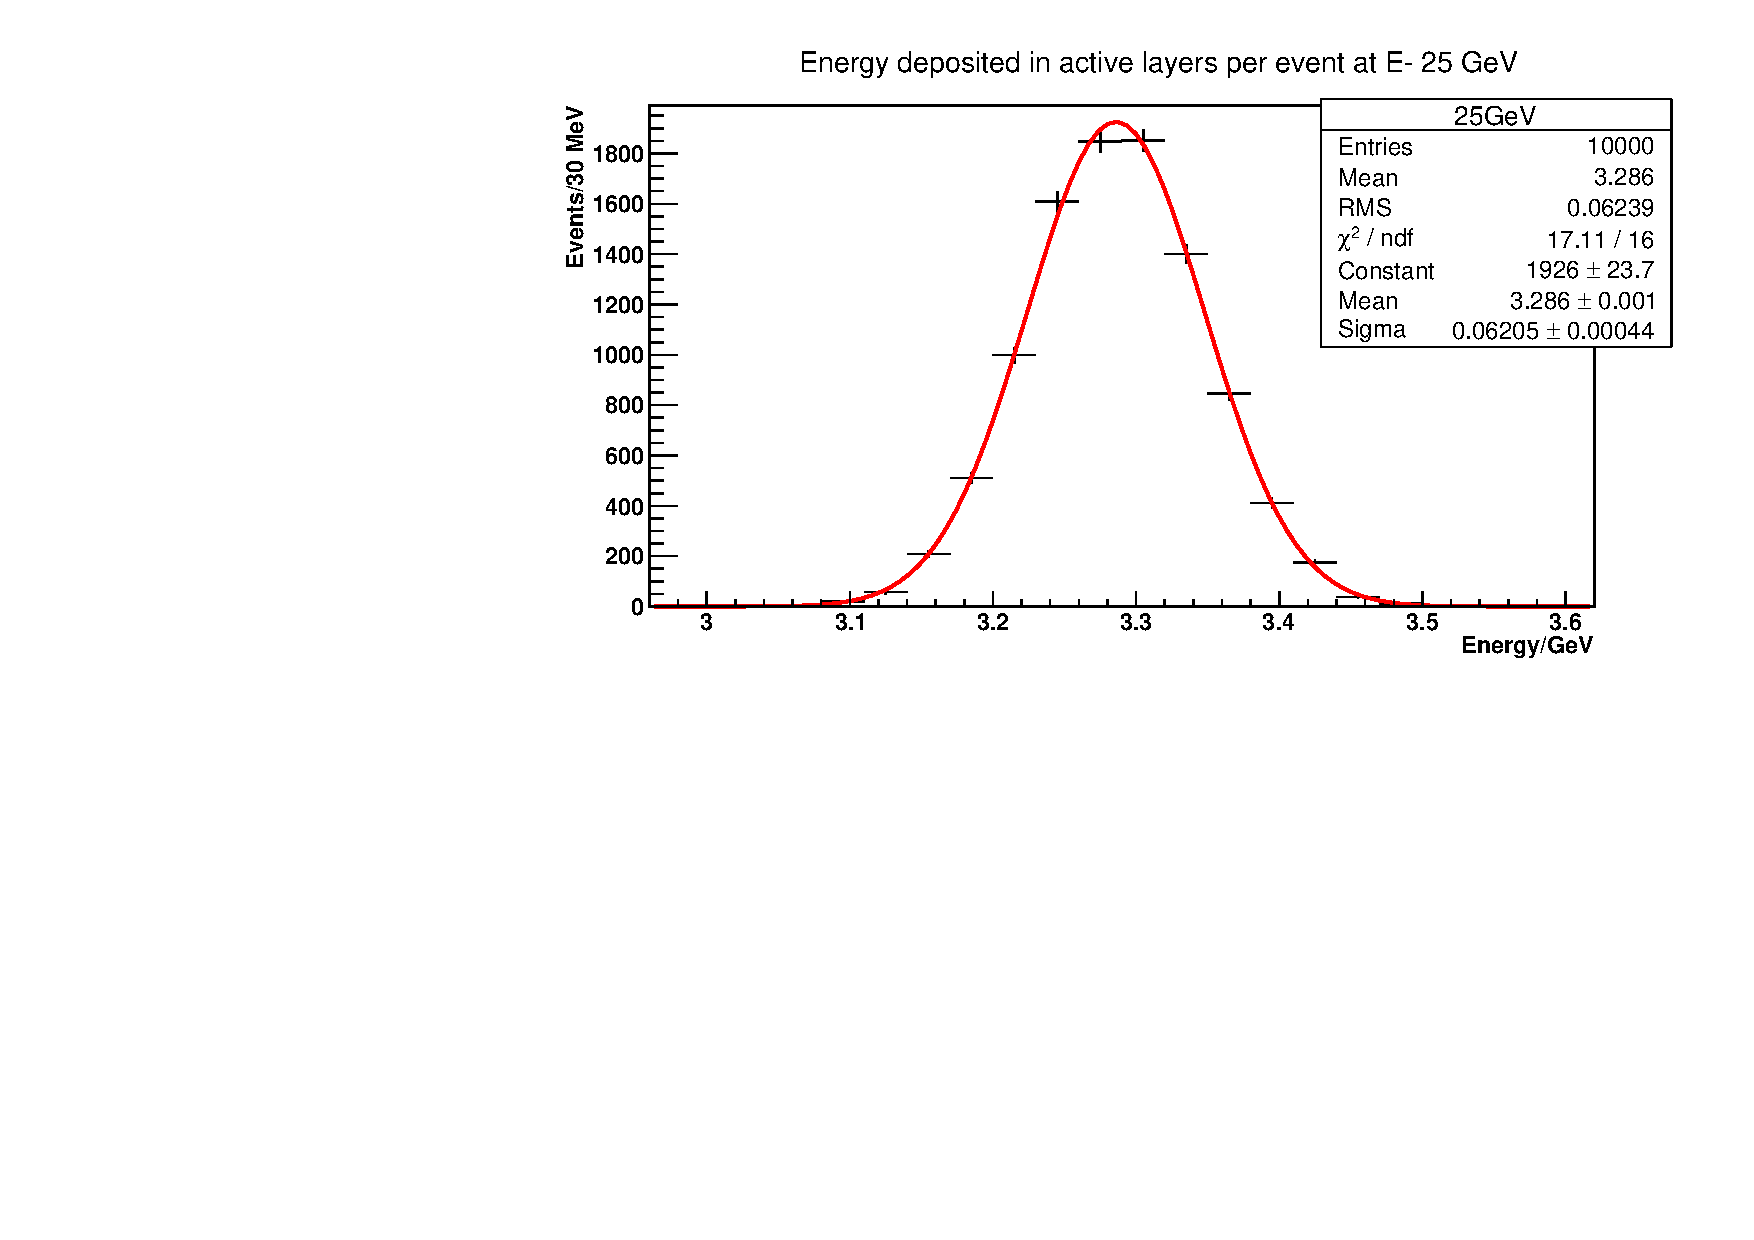
\includegraphics[width=\textwidth]{GaussExample.pdf}
  \caption{The distribution of energy deposited in scintillator(active) layers at 25 GeV}
  \label{fig:Gauss}
\end{figure}

From these fits the standard deviation divided by the mean was plotted against the incident particle energy, as defined in the configuration of \geant.  $\frac{\sigma}{E}$ is expected to follow equation \ref{eq:fr} but without the b term. Therefore a mimimum chi squared fit to,
\begin{equation}
  \label{eq:fitfr}
  \frac{\sigma}{E}=\frac{a}{\sqrt{E}}\bigoplus c
\end{equation}
was performed with the parameters 'a' and 'c' left floating as these are to be determined by the fit.  This process was applied to both \geant version 9.5.p02 and 9.6.p04 with the same energies and 10000 events at each energy.  The results of these fits for both \geant versions are shown in figure \ref{fig:straightres} and table \ref{tab:results}.
\begin{figure}[h]
  \centering
  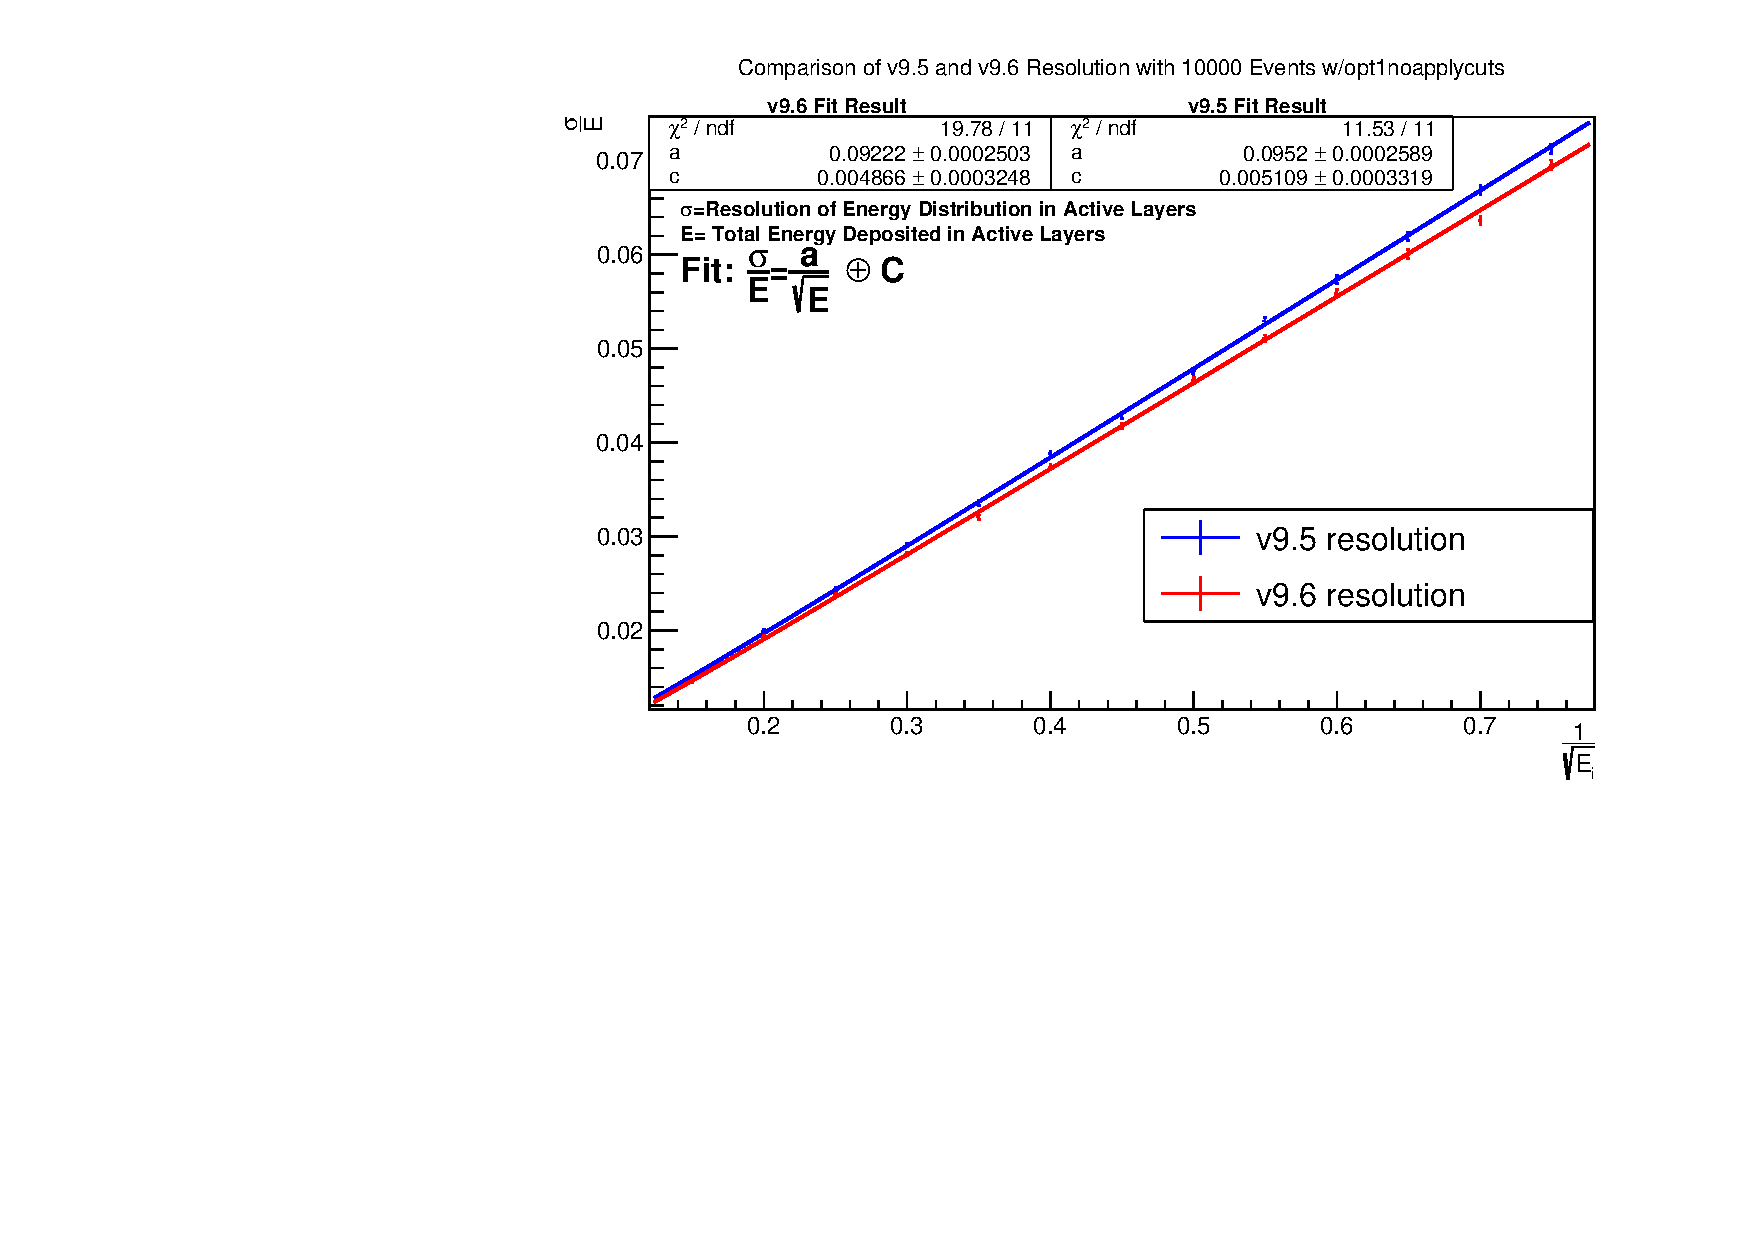
\includegraphics[width=\textwidth]{StraightCompareUse.pdf}
  \caption{A plot of fractional resolution against $\frac{1}{\sqrt{E}}$ comparing versions of \geant. The fit is the function given in equation \ref{eq:fitfr}.}
  \label{fig:straightres}
\end{figure}
%\begin{figure}[h]
 % \centering
  %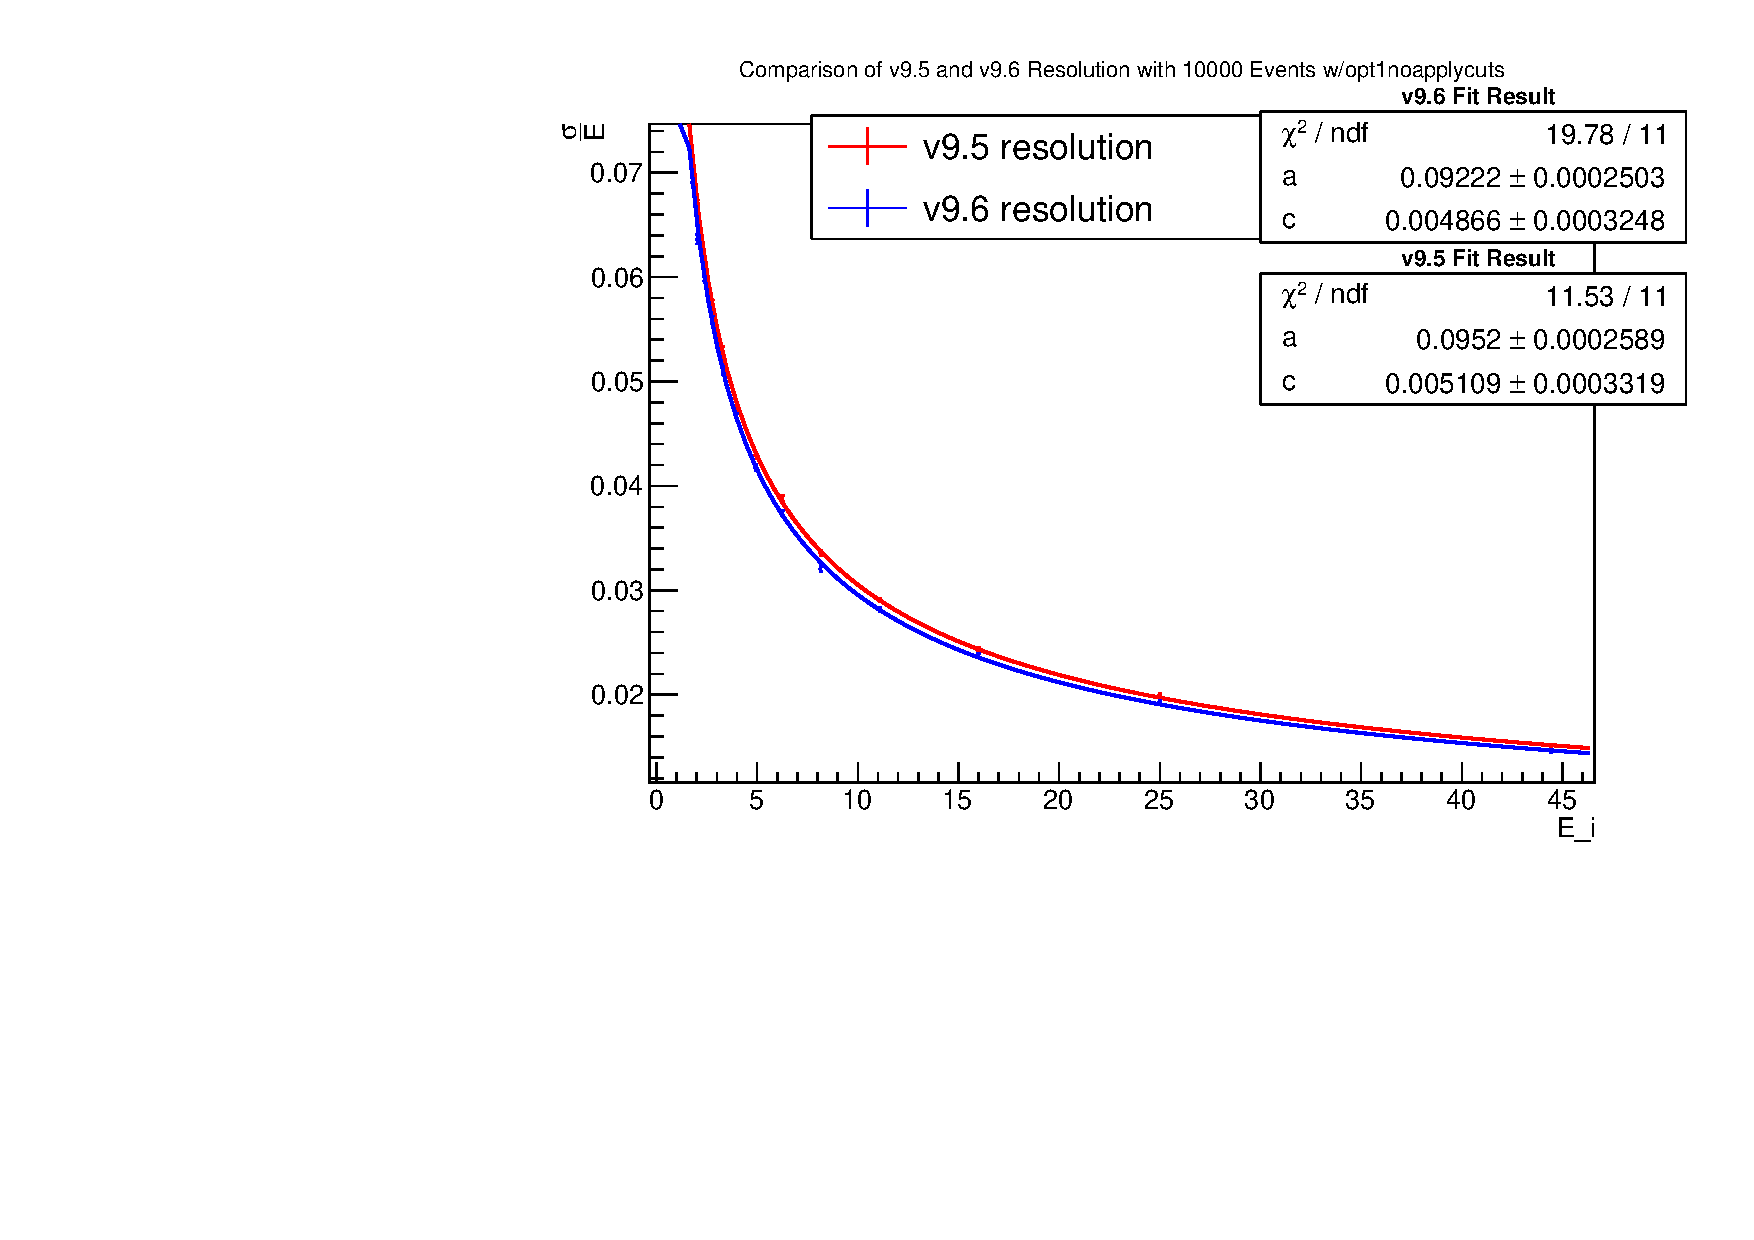
\includegraphics[width=\textwidth]{CurvedCompare.pdf}
  %\caption{A plot of fractional resolution against $E$ comparing versions of \geant. The fit is the function given in equation \ref{eq:fitfr}.}
  %\label{fig:coolres}
%\end{figure}

\begin{table}[h]
  \centering
  \begin{tabular}{|c|c|c|c|}
      \hline
      Version: & v9.5 & v9.6 & Difference  \\ \hline
      A term    & 0.0952$\pm$0.0003 & 0.0922$\pm$0.0003  & 8.43$\sigma$, 3.3\% \\ \hline
      C term    & 0.0051$\pm$0.0003 & 0.0049$\pm$0.0003 & consistent \\ \hline
      $\frac{\chi^2}{ndf}$   &1.798  & 1.048 &  \\ \hline
  \end{tabular}
  \caption{Fractional resolution results for comparison of \geant versions.  These results are obtained from the fits shown in figures \ref{fig:straightres}}
  \label{tab:results}
\end{table}

It is clear from these fits that there is a significant discrepancy in the statistical term of the fractional resolution parameterisation between \geant versions, despite the same PL being used in both versions.  The simulation of electromagnetic showers is a well established process that, in general, shows good agreement with data.  Therefore, progression of results this significant is not expected.  As many different processes contribute to electromagnetic showering more investigations were needed to understand exactly which part of the simulation is giving rise to this discrepancy.

\paragraph{Sampling Fraction and Shower Profile Investigations}
\label{sec:Sampling Fraction and Shower Profile Investigations}
In order to understand the unexpected results described in section \ref{sec:Fractional Resolution Investigation} it was decided that a study of the shower profiles in both active and passive layers of the calorimeter would be performed.  A shower profile is a plot of dE/dX against X, where X is the longitudinal depth from the front face of the calorimeter and E is the energy deposited.  Although X is often expressed in terms of radiation lengths, in this case the layer number was used because the shower profiles were in bins corresponding to the thickness of one layer of the ECAL.

Again, electrons at 13 different energies between 1.78GeV and 44.44GeV were fired into the ECAL using both \geant versions.  At each energy, shower profiles for active and passive layers were considered seperately and the profiles resulting from each version of \geant were plotted on top of each other for comparison.  The results at 1.78GeV and 44.44 GeV are shown in figures \ref{fig:1.78sp} and \ref{fig:44.44sp} respectively, all other energies are shown in \ref{ap:sp}.
\begin{figure}[h]
  \centering
  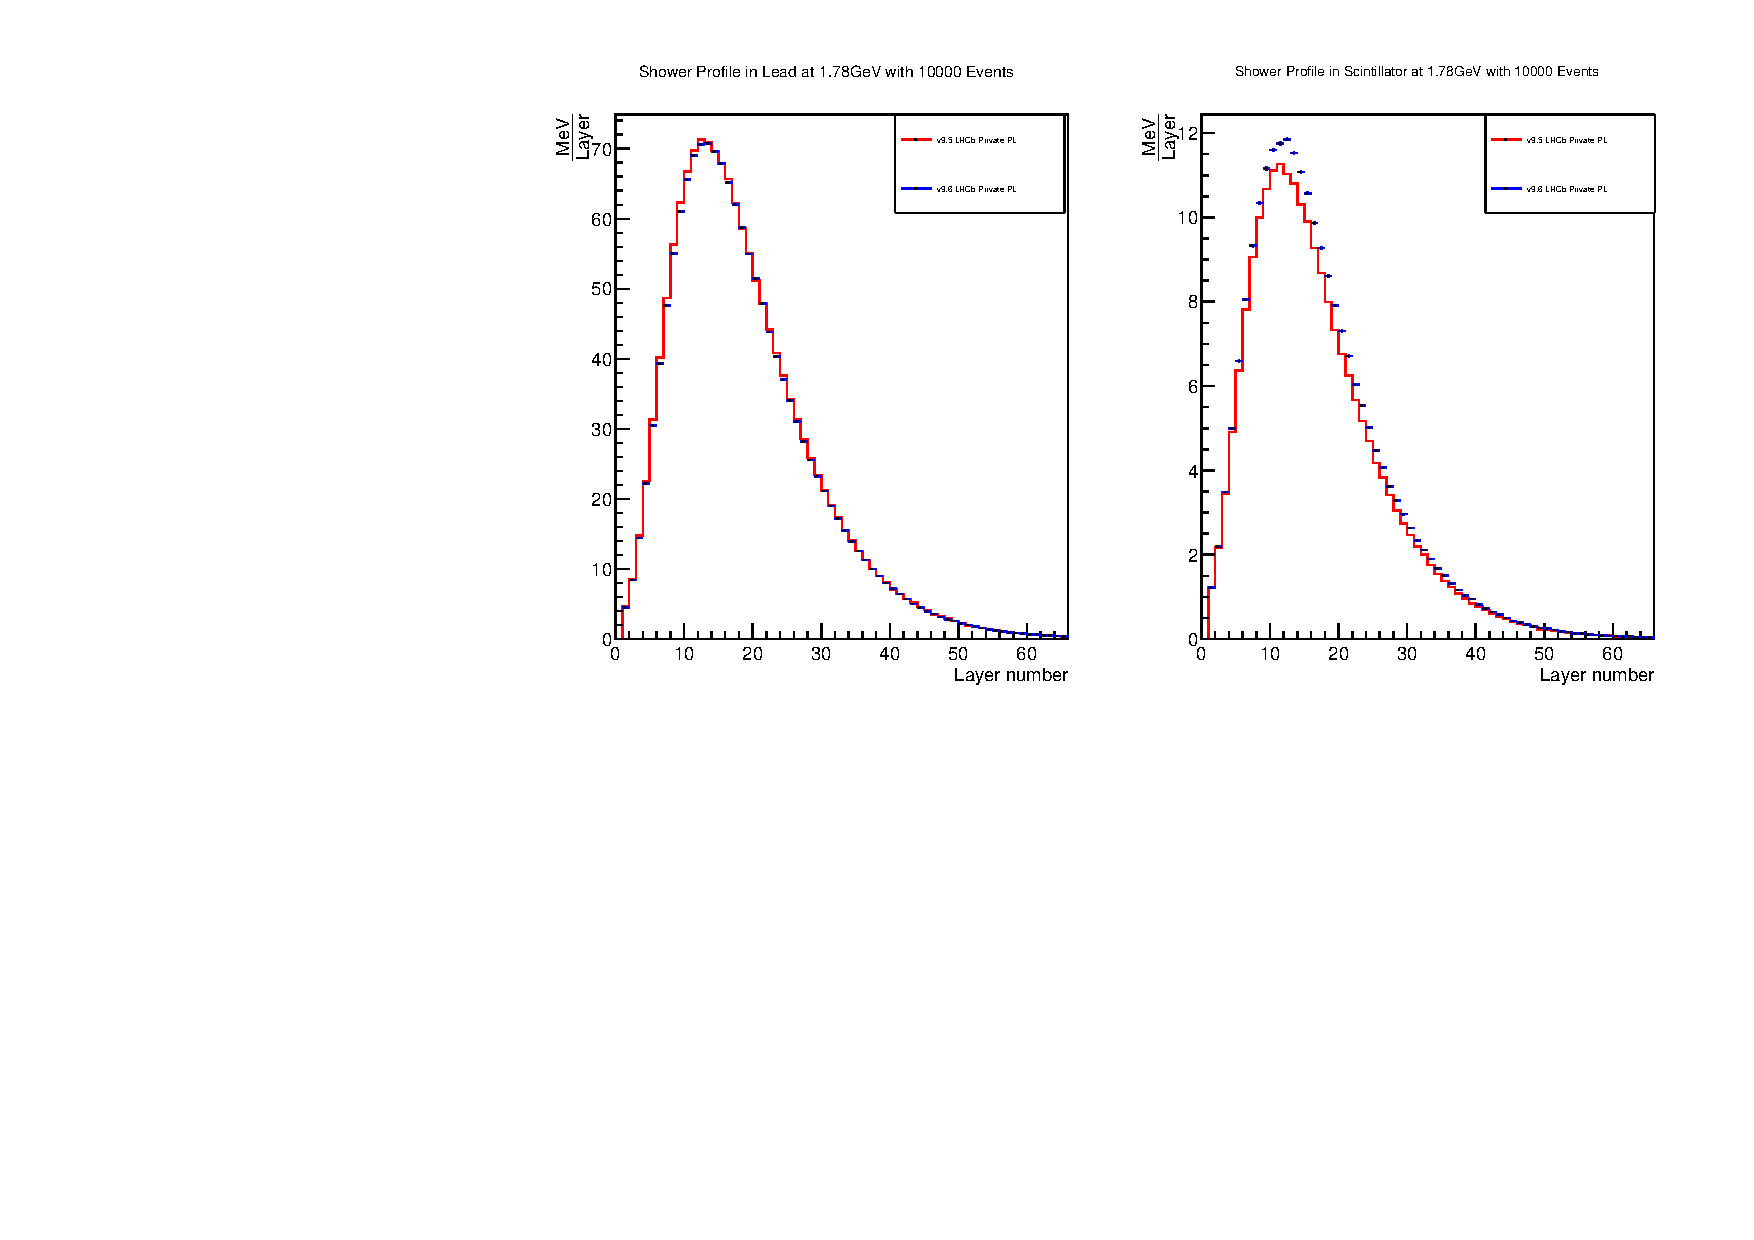
\includegraphics[width=\textwidth]{ShowerProfiles178.pdf}
  \caption{A comparison of shower profiles between \geant version 9.5 and 9.6 using the \lhcb private physics list for 1.78GeV electrons.  These profiles are normalised.}
    \label{fig:1.78sp}
\end{figure}
\begin{figure}[h]
  \centering
  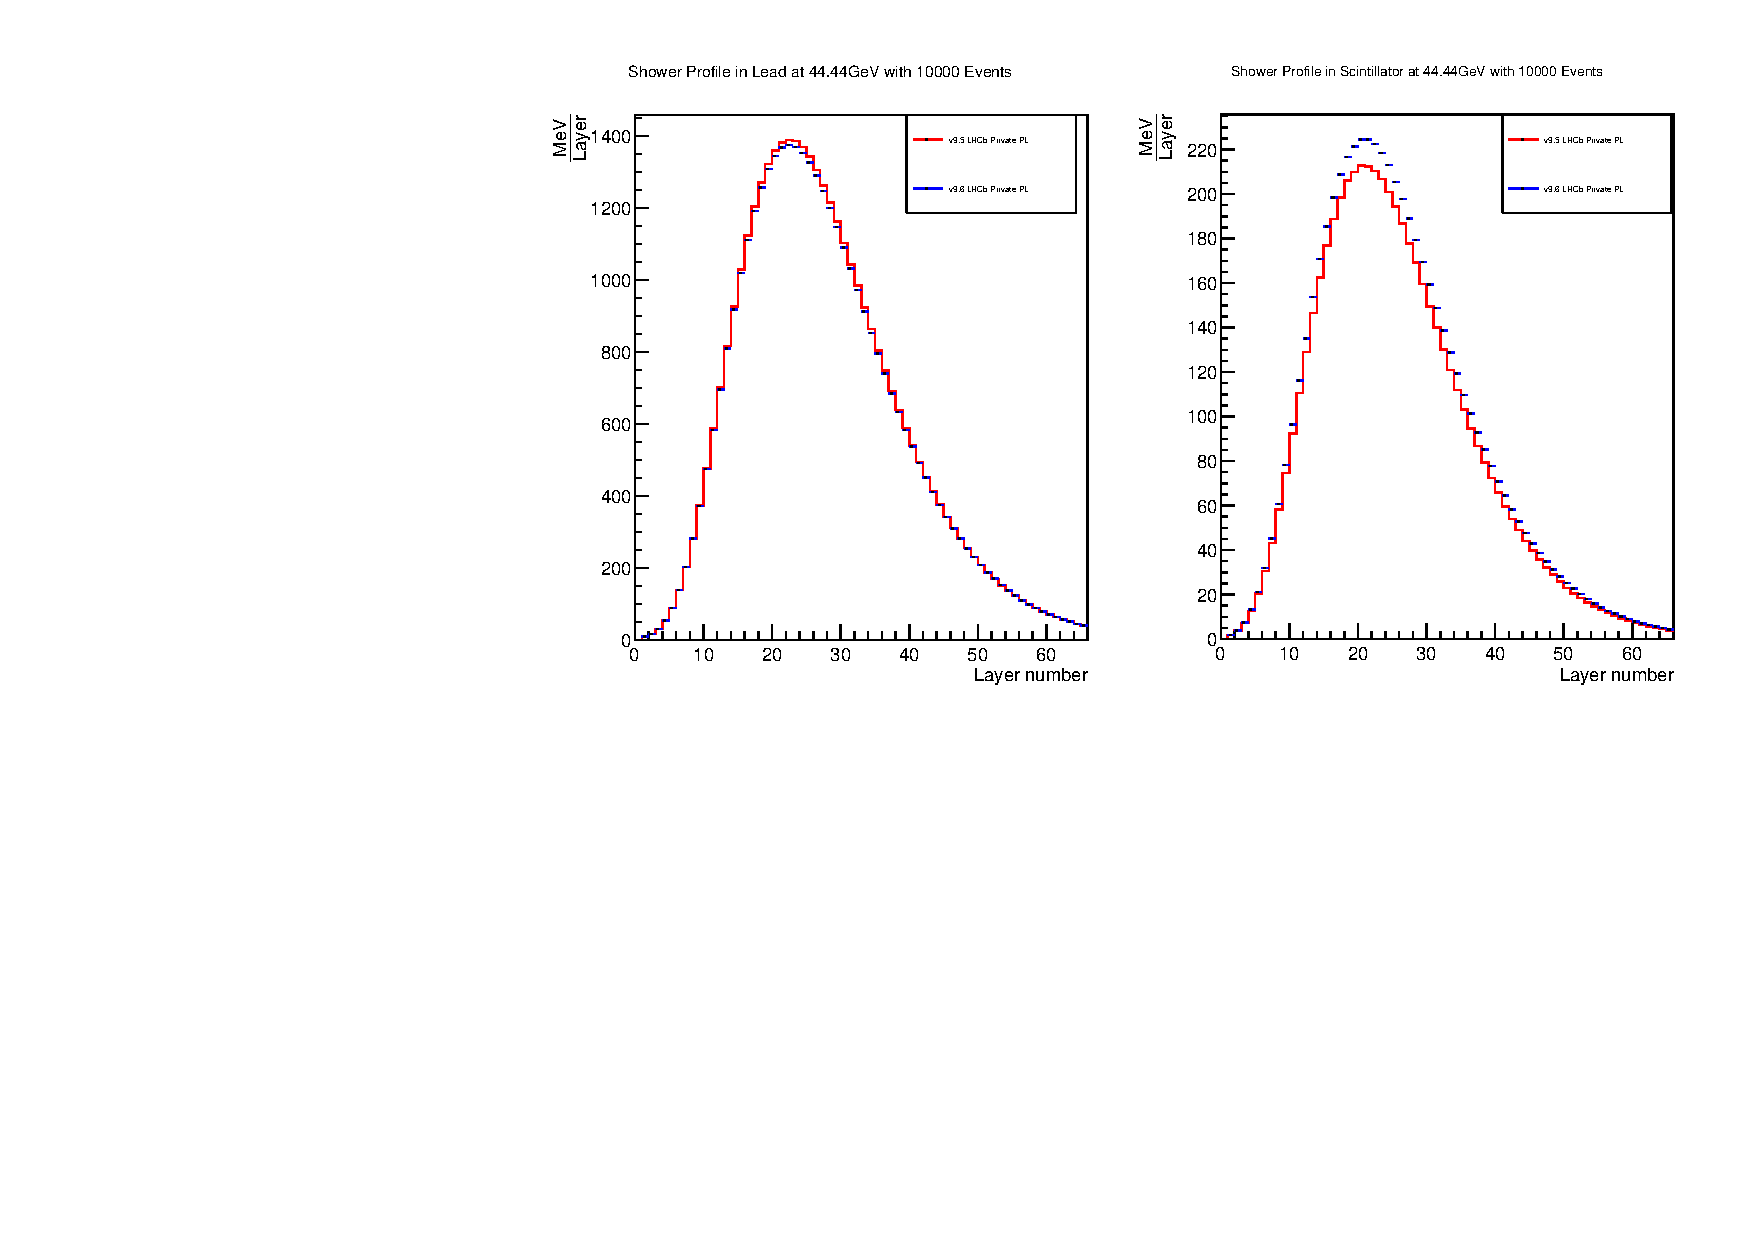
\includegraphics[width=\textwidth]{ShowerProfiles44.pdf}
  \caption{A comparison of shower profiles between \geant version 9.5 and 9.6 using the \lhcb private physics list at 44.44GeV electrons. These profiles are normalised.}
    \label{fig:44.44sp}
\end{figure}

It is clear from these shower profiles that \geant version 9.6.p04 is depositing more energy in active layers and less energy in passive layers compared to \geant 9.5.p02.  This pattern is observed at all energies simulated.

%To further investigate this behaviour the shower profiles were split by particle type; seperate shower profiles were plotted for electrons, positrons and photons.  These results can be seen in figures \ref{fig:1.78spseperate}  and \ref{fig:44.44spseperate}.
%PUT SEPERATE SHOWER PROFILES HERE
%These reuslts show that the observed discrepancy can not be attributed to the way in which photons are modelled because the total energy deposited by photons is negligable and would therefore not be able to influence the overall shower profiles.

In order to quantify further this observed change in behaviour, the ECAL sampling fraction as a function of energy was studied for both \geant versions.  The sampling fraction, in this context, is defined as the energy deposited in active layers (visible energy) divided by the incident particle energy.  The total energy deposited in each type of material was obtained by integrating the shower profiles over all layers.  The resulting sampling fraction as a function of energy is shown in \ref{fig:sfcomp}.
\begin{figure}[h]
  \centering
  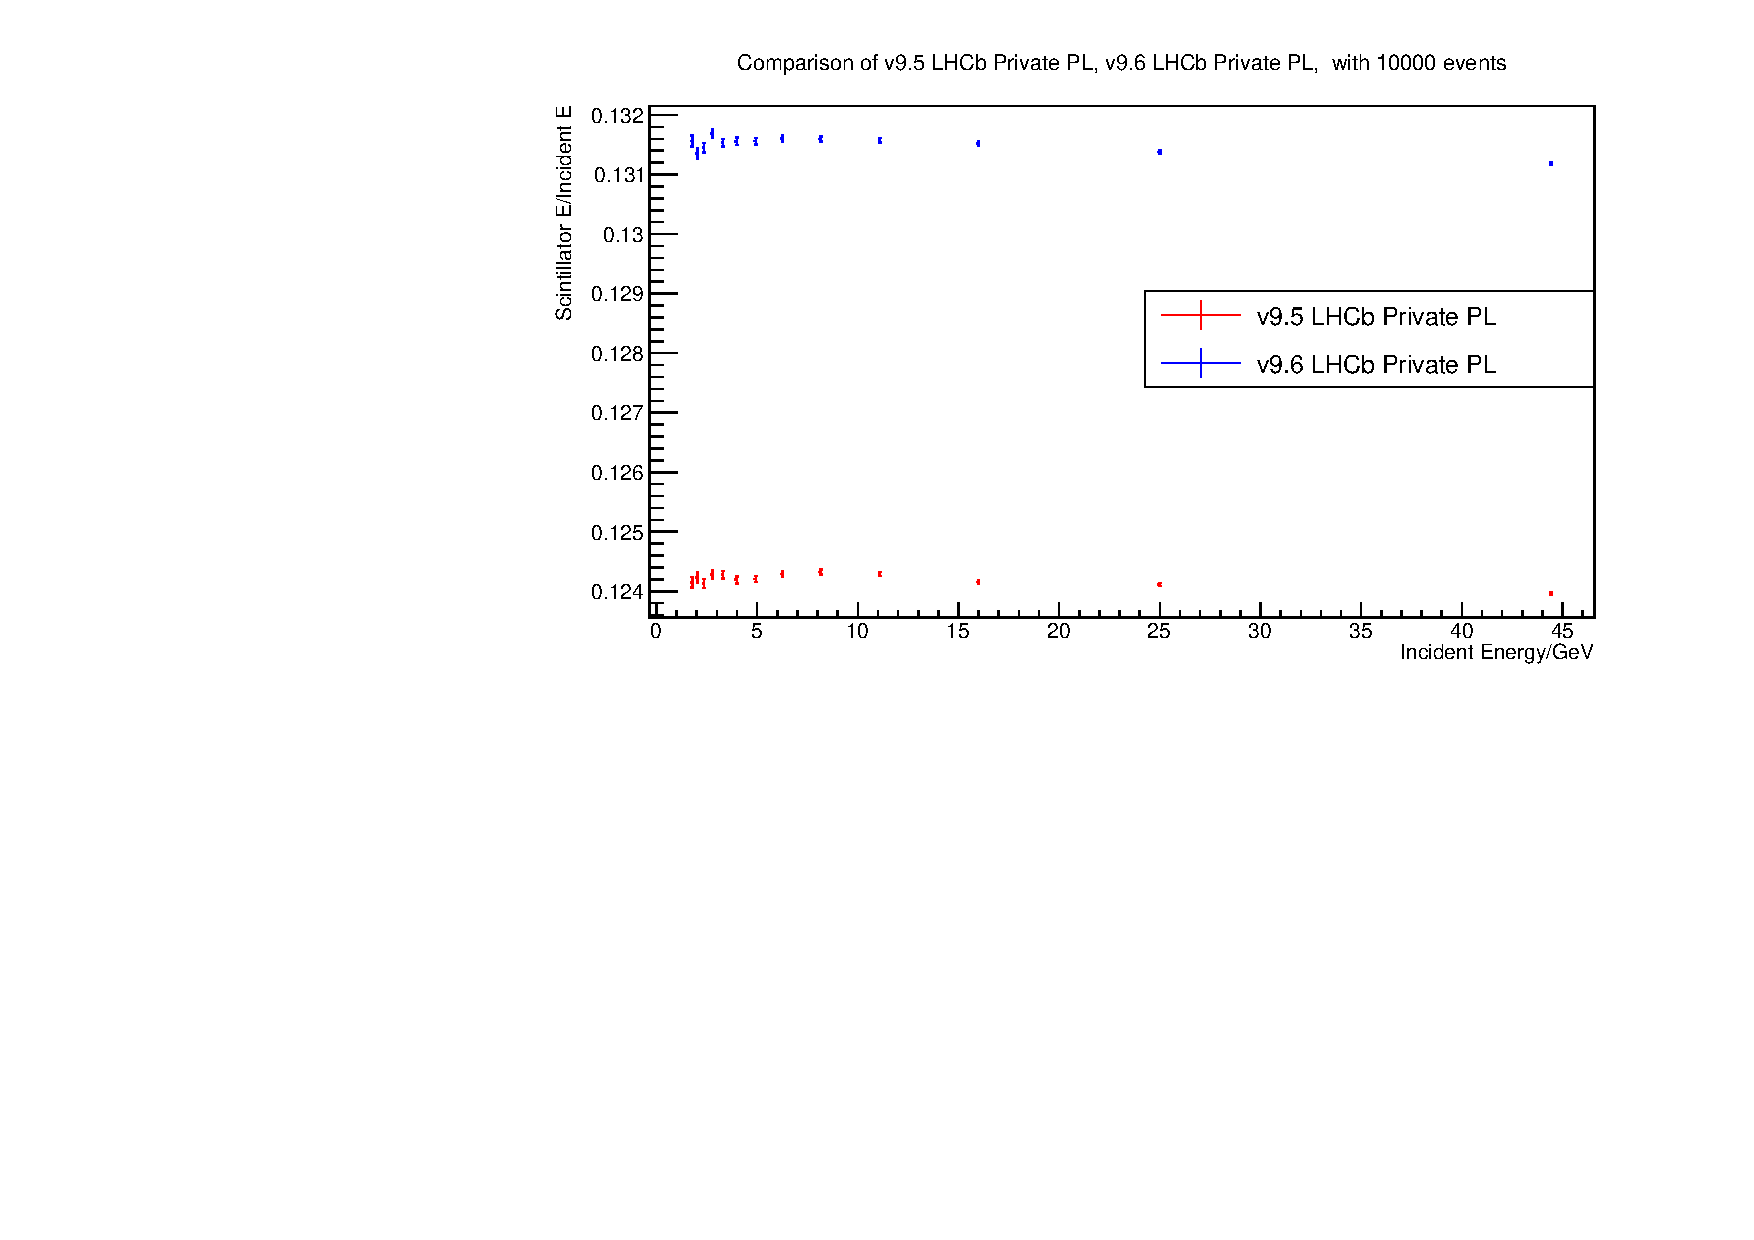
\includegraphics[width=\textwidth]{SamplingFractionVersions.pdf}
  \caption{A plot of sampling fraction as a function of energy for both versions of \geant}
  \label{fig:sfcomp}
\end{figure}
To further this quantification the ratio of energy deposited in active layers to passive layers was also plotted as a function of energy for both \geant versions and the results are shown in figure \ref{fig:ratiocomp}.
\begin{figure}[h]
  \centering
  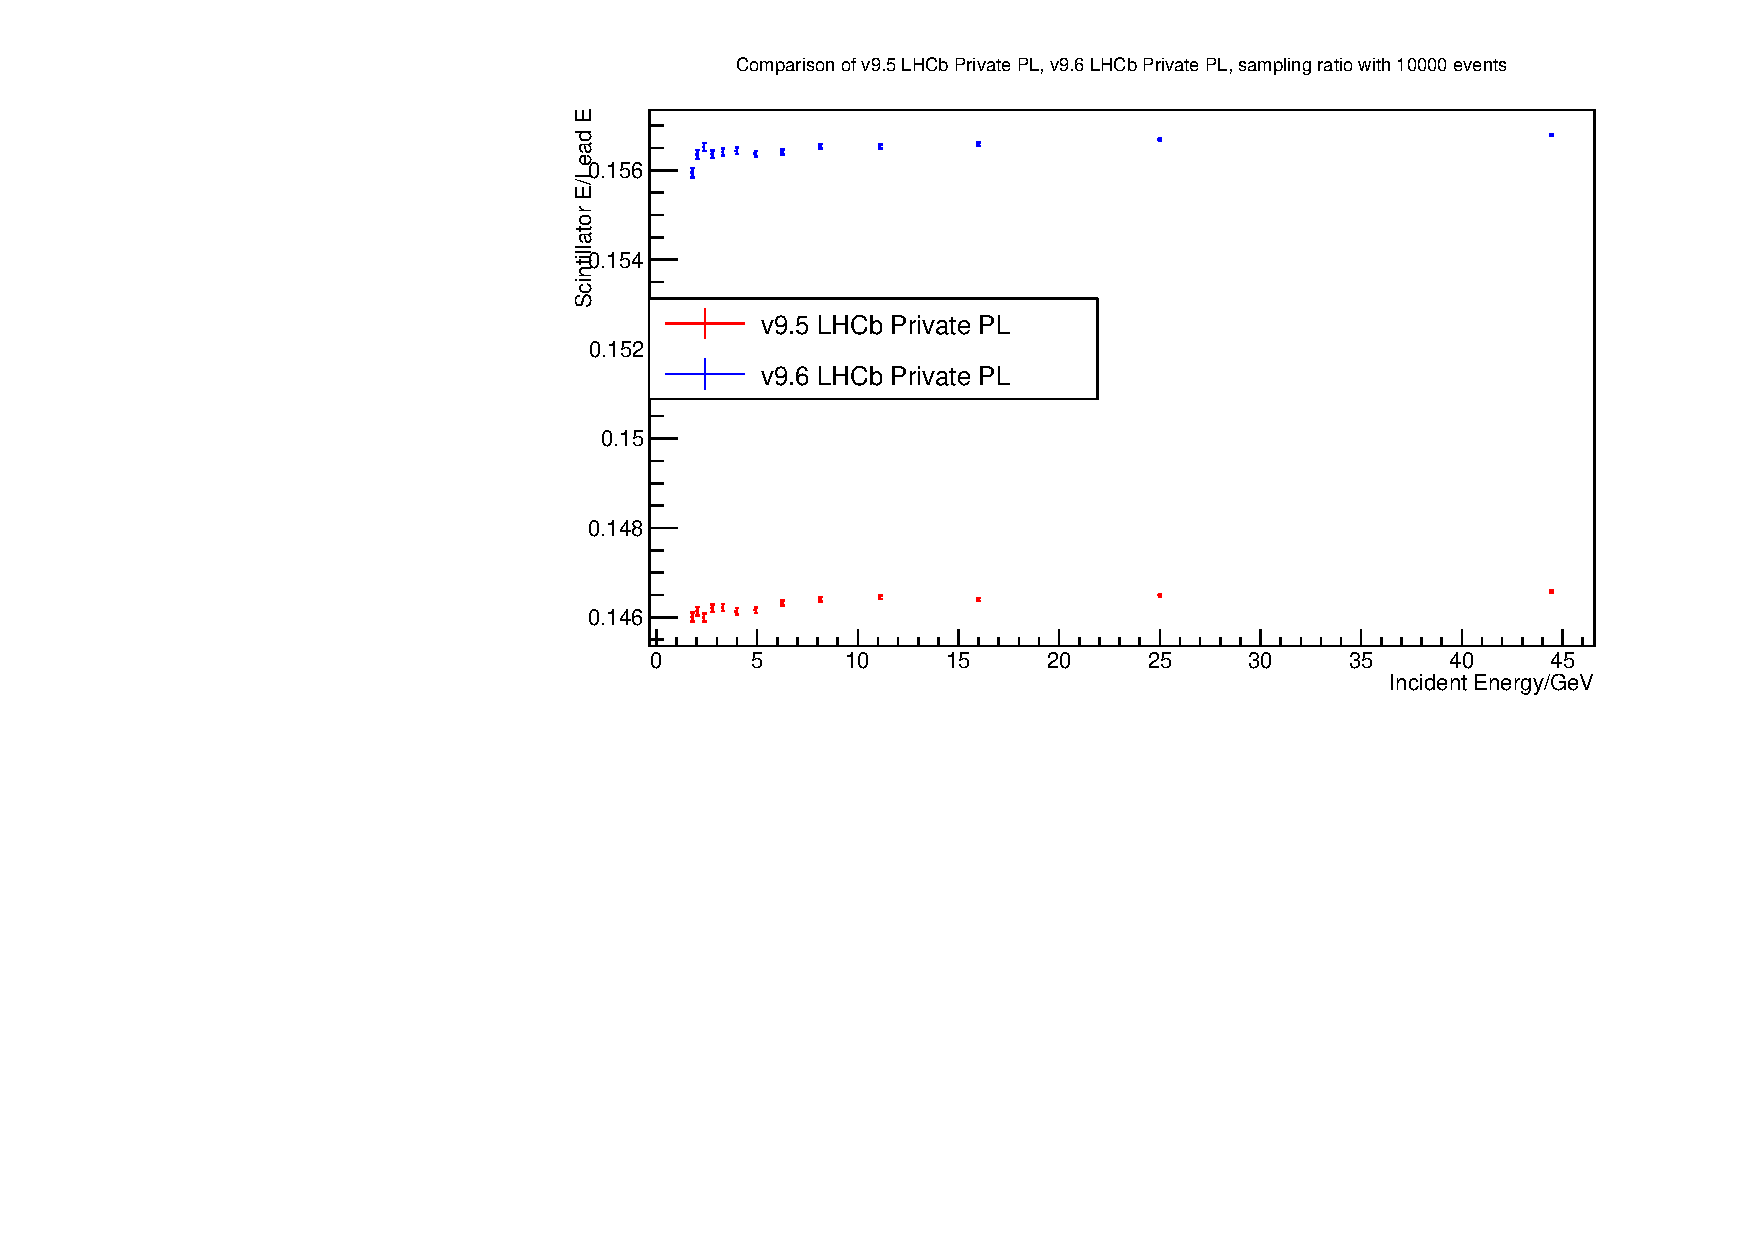
\includegraphics[width=\textwidth]{SamplingRatioVersions.pdf}
  \caption{A plot of the ratio of energy deposited in active layers to passive layers as a function of energy for both \geant versions}
  \label{fig:ratiocomp}
\end{figure}
The results from the investigation of sampling fraction and sampling ratio are summarised in table \ref{tab:sfcomp}.

\paragraph{Discussion of results for \geant version comparison}
\label{sec:Discussionofresultsone}
The results of these sampling fraction studies are significant, both statistically and in terms of the implications for the next simulation package used by \lhcb.  It is very clear that the sampling fractions have changed between \geant versions and this change would explain the observed discrepancy in fractional resolution seen in section \ref{sec:Fractional Resolution Investigation}.  Sampling more energy would always improve the fractional resolution of an ECAL because it means any statistical fluctutations are relatively less significant. The ECAL has to be calibrated in monte carlo such that an observed value of visible energy corresponds to the correct incident energy.  Since these results show that the visible energy of the ECAL has changed in this new version of \geant this calibration will have to be performed again when the new simulation package is released.

The precise cause of these discrepancies needs to be understood because there could be implications for the simulation of other detector components.  Therefore, the models used when the \lhcb PL is specified were compared between versions and the following changes were consider possible causes of the discrepancy:
\begin{itemize}
\item \textit{New implementation of UrbanMsc95 multiple scattering model.}  It is detailed in the release notes that sampling of multiple scattering in version 9.6 is now performed before the energy loss of each particle.  However, in version 9.5 and before energy loss was sampled before multiple scattering.  If this changed the scattering andlge distribution of electrons and positrons in the calorimeter, it could change the number of particles that scatter over the boundary between active and passive layers.
\item \textit{Change in angular distribution model for electron bremsstrahlung.} In version 9.6 a boosted dipole approximation is used for the angular distribution of photons emitted in electron bremmsstrahlung, as described in \cite{:/content/aip/journal/apl/80/17/10.1063/1.1473684}.  A change in the angular distribution of bremsstrahlung could also result in particles previously depositing energy in passive layers traversing the boundary between layers and depositing energy in active layers instead.
\end{itemize}

After contacting the \geant collaboration, the cause of the observed discrepancy is believed to lie with the changes to the multiple scattering model.  In fact, the \geant collaboration recommended that the multiple scattering models used in the \lhcb private PL are changed from \textit{UrbanMsc95} to \textit{UrbanMsc93} below 100MeV and \textit{WentzelVI} above 100MeV.  This would bring the simulation of multiple scattering within the LHCb private PL inline with the \geant \textit{emstandard opt1} physics list.
\clearpage
\subsubsection{Comparison of Physics Lists}
\label{sec:Comaprison of PL}
As the \geant collaboration had recommended a change to the LHCb private PL it was decided a thorough investigation of other PL options would be carried out using the simple calorimeter test.  This would be done using \geant version 9.6.p04, so that investigations directly related to the next version of the \lhcb simulation package could be carried out.  The results of these investigations would help to inform the decision of which PL to use for the next release of \gauss.  

The following physics lists supplied by \geant were investigated:
\begin{itemize}
\item \textit{emstandard option0}
  This is the default electromagnetic phyics list used by \geant (in general).  This is designed to give optimal accuracy at medium and high energies, which are the typical energies present at HEP experiments.  In version 9.6 this PL uses the \textit{UrbanMsc95} multiple scattering model.
\item \textit{emstandard option1}
  This physics list is designed for HEP experiments but is described as \cms focused. This PL has moved back to using the \textit{UrbanMsc93} multiple scattering model below 100MeV and the WentzelVI model above 100MeV in version 9.6.  It also uses the \textit{minimal} step limit type which applys looser limitations on the maximum length of a single simulation step.  This results in less steps being simulated, leading to large savings in CPU time.  However, this is known to cause bias in the results and this bias increases for longer production cuts \cite{1742-6596-219-3-032045}.
\item \textit{emstandard option2}
  This physics list is also designed for HEP experiements but is described as \lhcb focused.  It uses the \textit{UrbanMsc93} multiple scattering model and uses a different angular distribution generator for bremsstrahlung.  Like \textit{opt1} it also uses the \textit{minimal} step limit type to save CPU time at the expense of accuracy.
\item \textit{emstandard option3}
  This PL provides the best accuracy of charged particle tracking in the absence of a magnetic field.  It uses the \textit{UrbanMscModel96} for multiple scattering.
\item \textit{emstandard option 4}
  This PL, like option 3, is designed to provide the best accuracy for charged particle tracking in the absence of a magnetic field and also uses the \textit{UrbanMscModel96} for multiple scattering.  However, it is designed to provide the highest accuracy at medium and low energies.
\end{itemize}

As well as the \geant supplied PLs there is also the \lhcb private physics list to consider.  This is simply \textit{emstandard option1} with the \textit{applycuts} option disabled.  However, it is based on the \textit{opt1} PL from \geant v9.4 which differs to both the v9.5 and v9.6 \textit{op1} PLs.  Therefore, rather than just updating the multiple scattering model used in the \lhcb private PL (as suggested by the \geant collaboration  and discussed in section \ref{sec:Discussionofresultsone}) it was decided that the new version of the \lhcb private PL would be the \textit{opt1} PL from v9.6 with the \textit{ApplyCuts} option disabled. Consequently, this study investigates both the old version of the \lhcb private PL (LHCbOld) and the new version (LHCbNew).

\paragraph{Fractional Resolution}
The first quantity used to test all the PLs described above was, again, the fractional resolution of the model ECAL.  Just as described in section \ref{sec:Fractional Resolution Investigation}, 10000 electrons were fired into the model ECAL at 13 different energies between 1.78GeV and 44.44GeV.  The same procedure as described in section \ref{sec:Fractional Resolution} was again used to extract $\frac{\sigma}{E}$ for each energy and a minimum $\chi^2$ fit to equation \ref{eq:fitfr} was performed to obtain the values of 'a' and 'c'.  The simulation was run with all of the PLs described in section \ref{sec:Comparison of PL}, allowing them to all be considered as a potential PL for the next version of \gauss.
\begin{figure}[h]
  \centering
  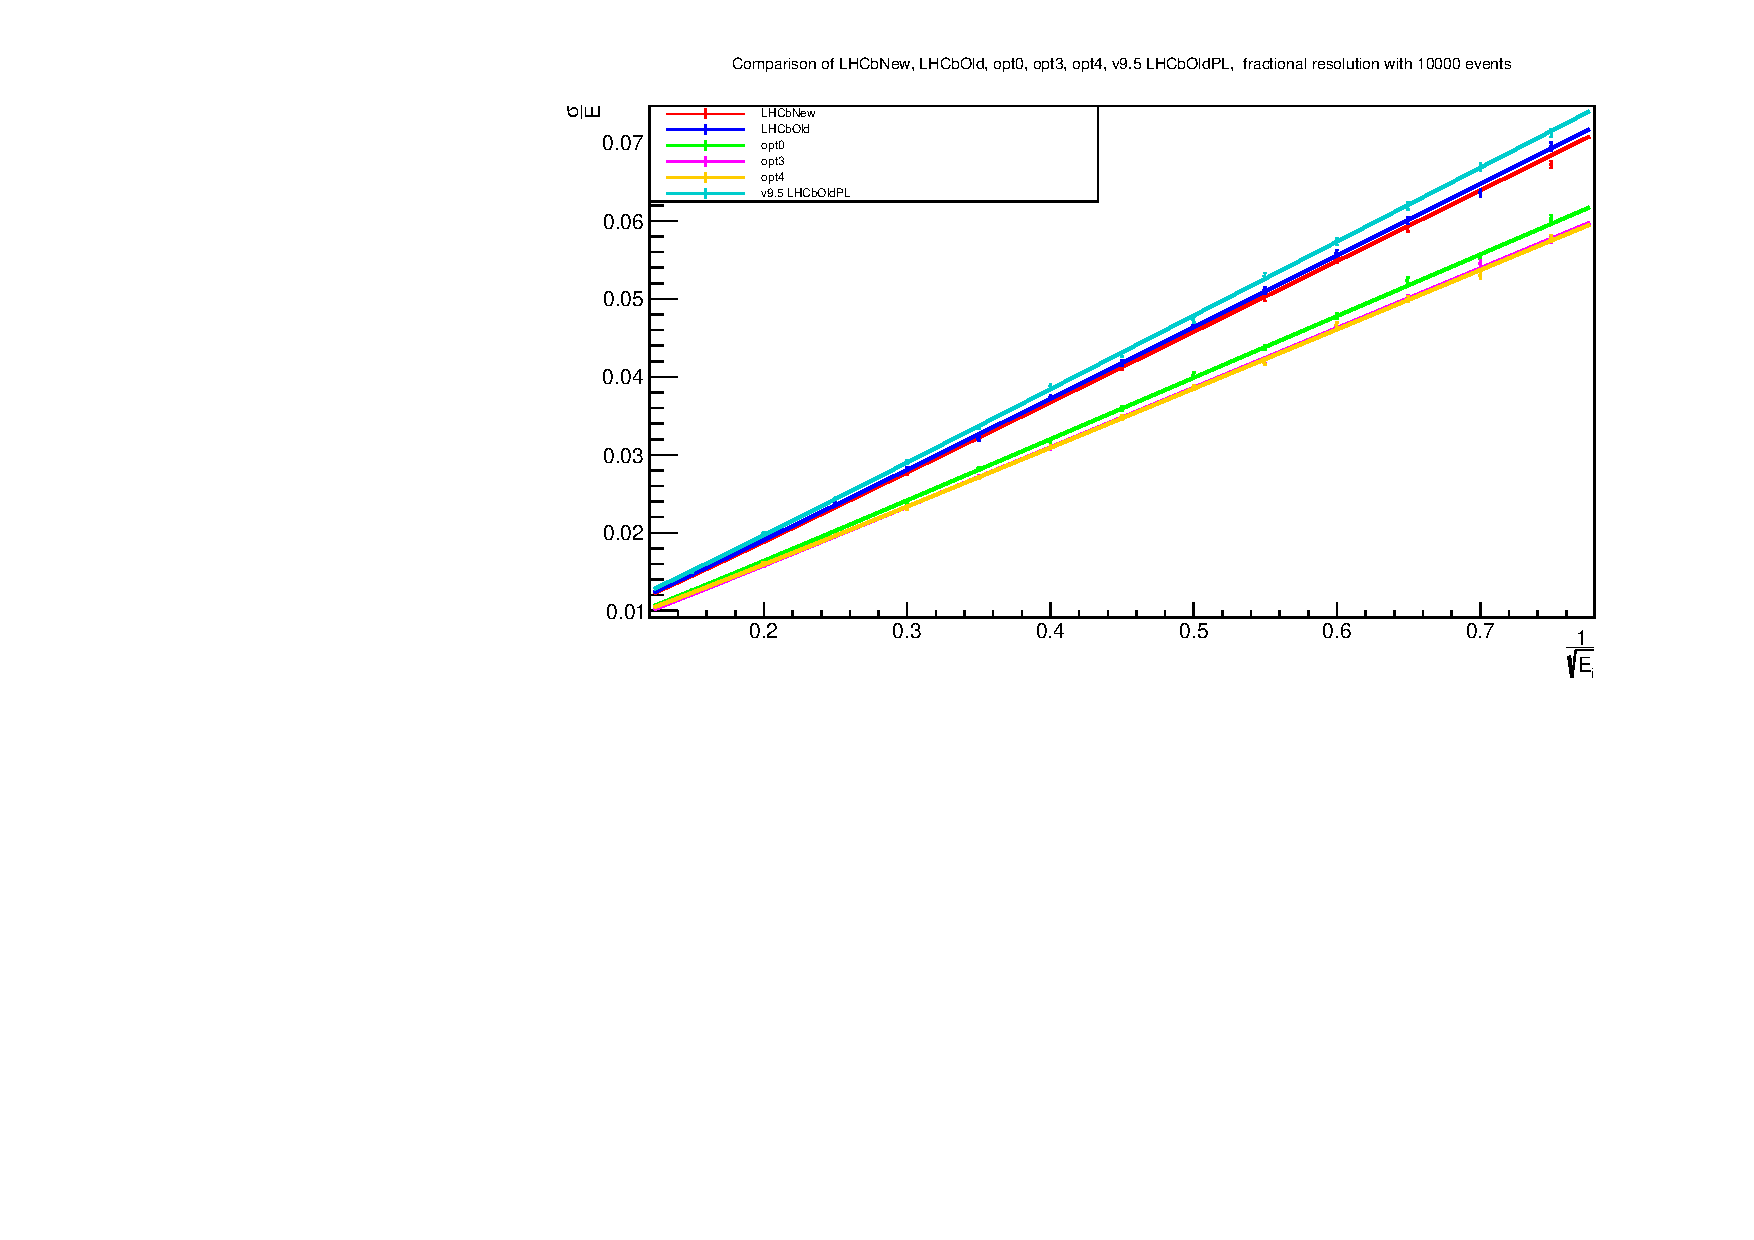
\includegraphics[width=\textwidth]{ProgressFR.pdf}
  \caption{A plot of fractional resolution against $\frac{1}{\sqrt{E}}$ for \geant v9.5 with the old PL and v9.6 with the new and old physics list options}
  \label{fig:LHCbPLStraightFR}
\end{figure}

Figure \ref{fig:LHCbPLStraightFR} shows the fractional resolution results with \lhcb private PLs, \textit{opt0},\textit{opt3} and \textit{opt4}, the result from \geant v9.5 is included for comparison.  A similar comparison is also made between all of the standard PLs supplied by the \geant collaboration, which is shown in Figure \ref{fig:BoxPLStraightFR}.  A summary of all fit results is shown in Table \ref{tab:AllPL}
\begin{figure}[h]
  \centering
  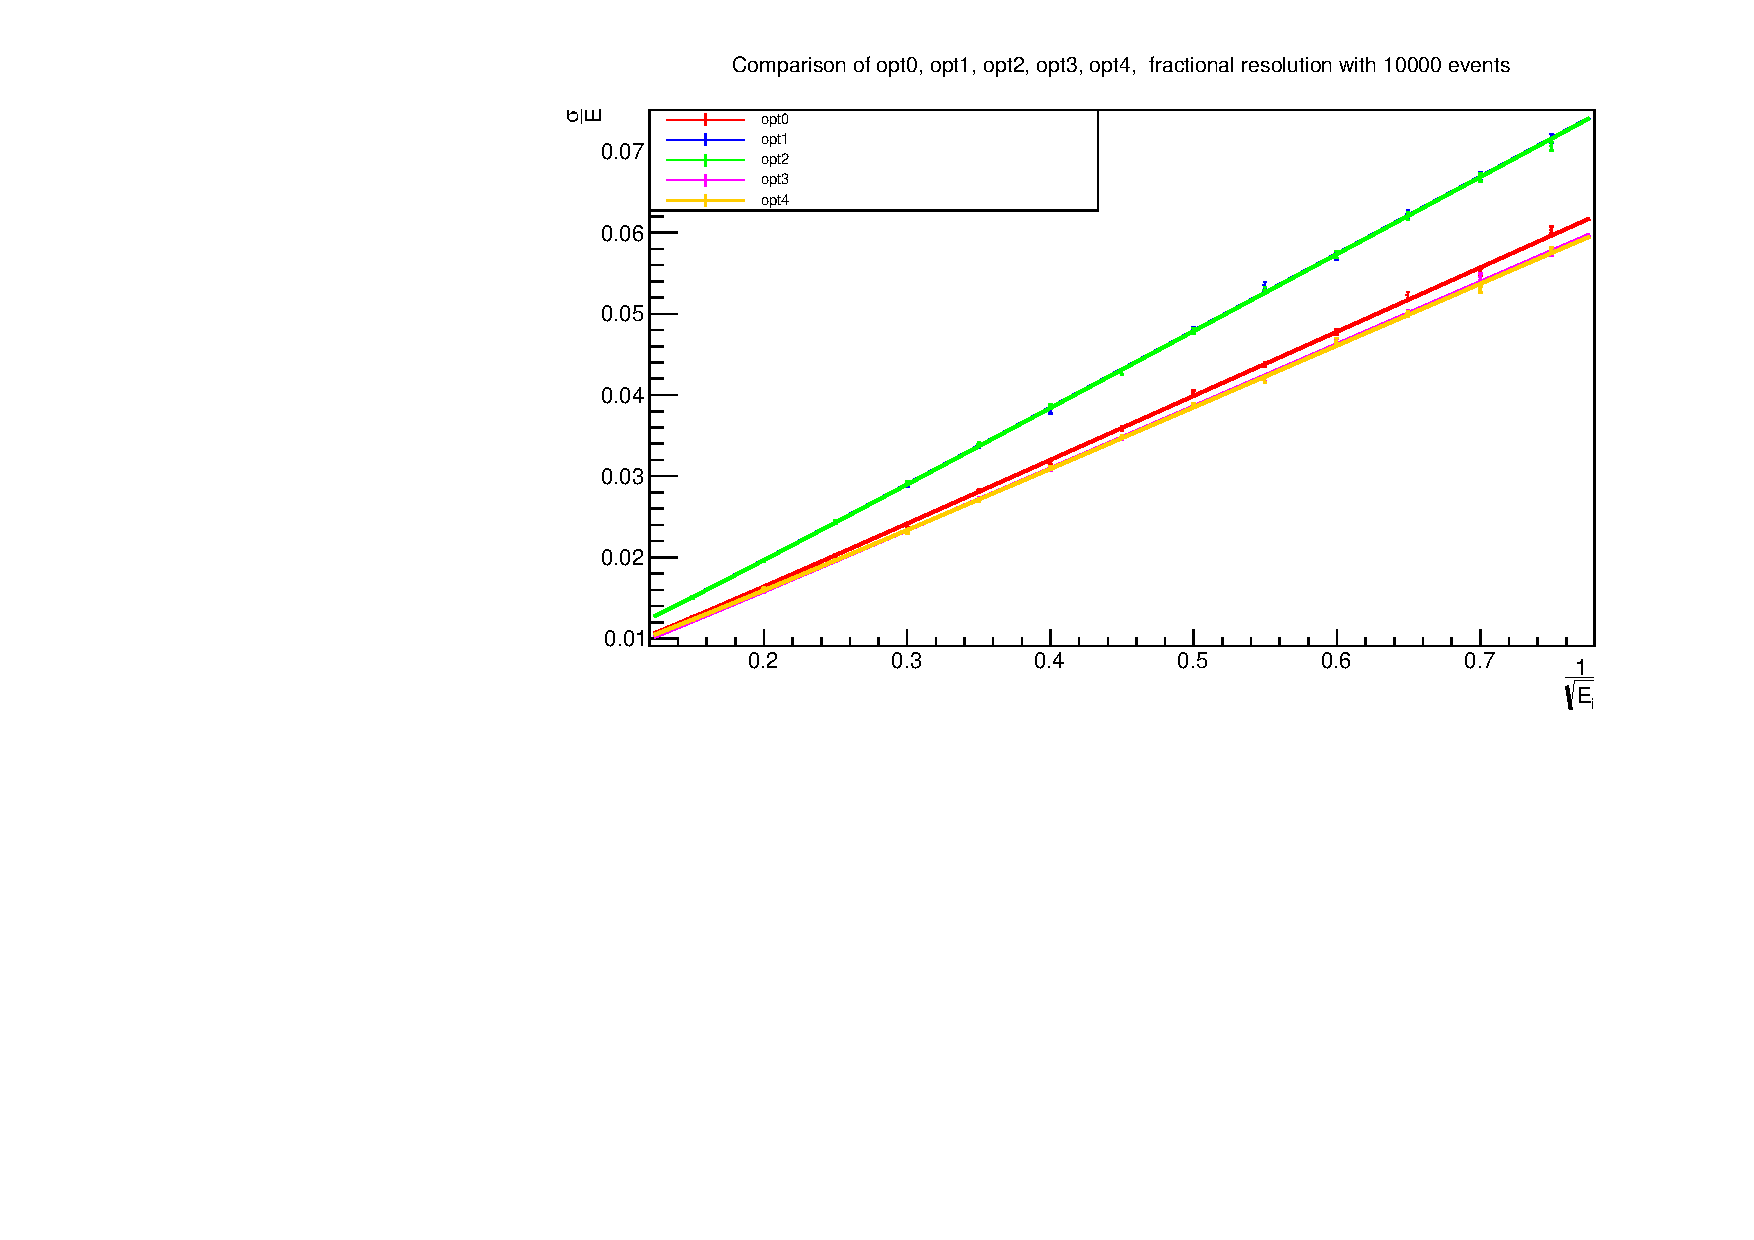
\includegraphics[width=\textwidth]{BoxStraightRes.pdf}
  \caption{A plot of fractional resolution against $\frac{1}{\sqrt{E}}$ for \geant v9.6 with all of the \textit{emstandard} PLs.}
  \label{fig:BoxPLStraightFR}
\end{figure}

\begin{table}[h]
  \centering
  \begin{tabular}{|c|c|c|c|}
      \hline
      PL & A term & C term & $\frac{\chi^2}{ndf}$  \\ \hline
      v9.5 LHCbOld & 0.0952 $\pm$ 0.0003 & 0.0051 $\pm$ 0.0003 & 1.05 \\ \hline
      LHCbOld & 0.0922 $\pm$ 0.0003 & 0.0049 $\pm$ 0.0003 & 1.80 \\ \hline 
      LHCbNew & 0.0910 $\pm$ 0.0002 & 0.0049 $\pm$ 0.0003 & 1.55 \\ \hline
      opt0 & 0.0794 $\pm$ 0.0002 & 0.0041 $\pm$ 0.0003 & 1.39 \\ \hline
      opt1 & 0.0953 $\pm$ 0.0003 & 0.0048 $\pm$ 0.0004 & 0.91 \\ \hline
      opt2 & 0.0953 $\pm$ 0.0003 & 0.0048 $\pm$ 0.0003 & 0.64 \\ \hline 
      opt3 & 0.0768 $\pm$ 0.0002 & 0.0037 $\pm$ 0.0003 & 0.67 \\ \hline 
      opt4 & 0.0764 $\pm$ 0.0002 & 0.0045 $\pm$ 0.0002 & 1.60 \\ \hline
  \end{tabular}
  \caption{Fractional resolution results for comparison of \geant physics lists.  These results are obtained from the fits shown in figures \ref{fig:LHCbPLStraightFR} and \ref{fig:BoxPLStraightFR}}
  \label{tab:results}
\end{table}

Figure \ref{fig:LHCbPLStraightFR} shows that updating the \lhcb private PL to follow \textit{emstandard opt1} has, in fact, increased the discrepancy with v9.5.  Although this initially seems troublesome, one should not necessarily expect the results from the new PL to match those of the old PL and \geant version because progression of results is expcected.  There is nothing to say the old PL would show the best agreement with data, in fact one should expect the newer version to be the most accurate.  It is, however, important that the progression of results is observed and calibrated for.

A direct comparison with data is not possible in this scenario due to limited test beam data and the absence of electronic noise in this simplifed scenario.   It is known that the \lhcb private PL has to use a simplified and consequently bias multiple scattering model due to CPU time constraints.  Therefore, the PLs that do not use a simplifed multiple scattering model (namely \textit{opt0}, \textit{opt3} and \textit{opt4}) should provide the best agreement with data and can consequently be used to check if progress towards greater accuracy has been made.  On this basis, Figure \ref{fig:LHCbPLStraightFR} shows that progress towards a more accurate fractional resolution result has been made by both moving to \geant v9.6 and updating the \lhcb private PL. Nevertheless, progress this large for well understood electromagnetic processes is still surprising.

Figure \ref{fig:BoxPLStraightFR} shows that there is a big difference in results between models that use a simplifed multiple scattering model and those that don't.  There is almost no difference between \textit{opt1} and \textit{opt2}, both of which \textbf{do} use a simplified multiple scattering model.  Likewise, \textit{opt3}, \textit{opt4}, and \textit{opt0} show results that are within $5\%$ of each other, all of which \textbf{do not} use a simpified multiple scattering model.  This is useful confirmation that, as expected and observed by \geant themselves, simplifying the multiple scattering model with the \textit{minimal} step limit option introduces bias to the result \cite{1742-6596-219-3-032045}.

\paragraph{Sampling Fractions and Shower Profiles} 
Using the same procedure as descirbed in section \ref{sec:Sampling Fraction and Shower Profile Investigations} shower profiles were created for all PLs under investigation.  
\begin{figure}[h]
  \centering
  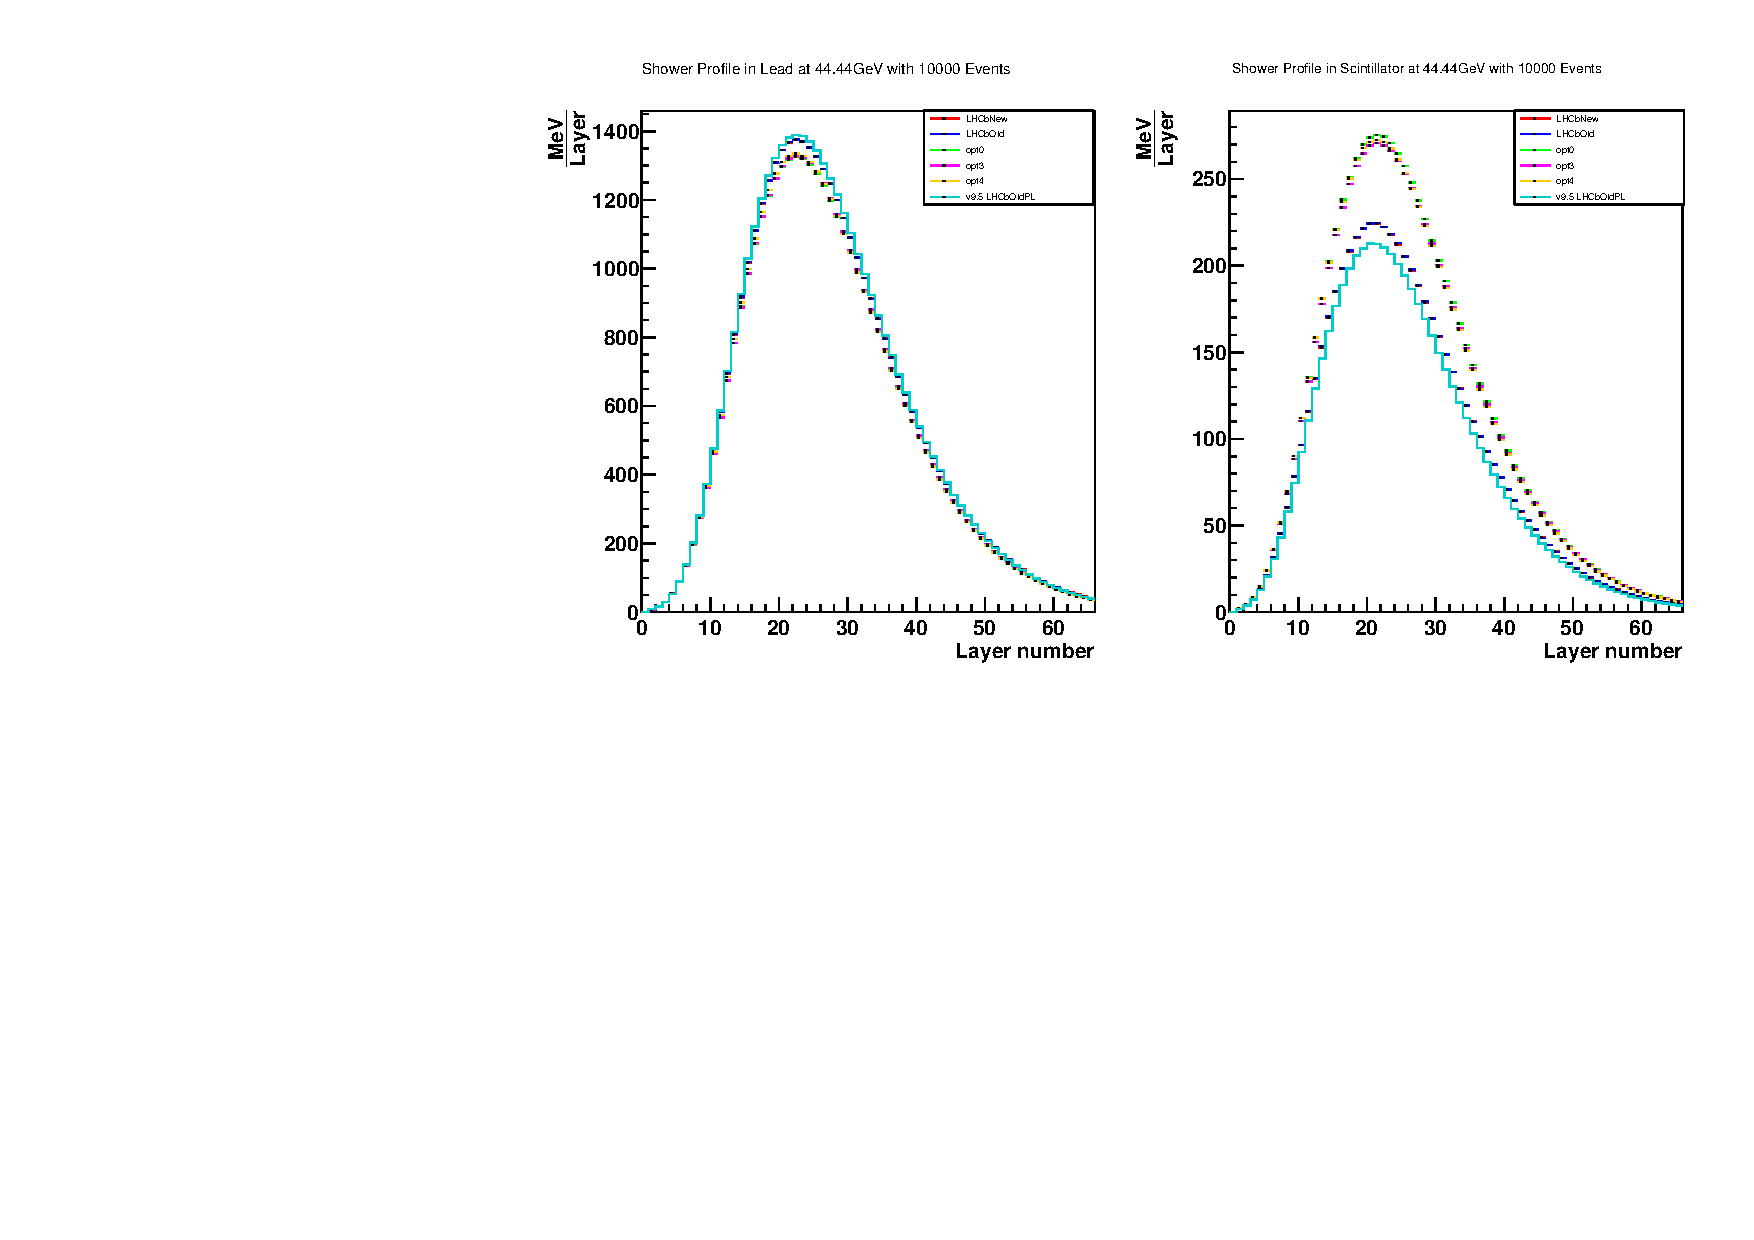
\includegraphics[width=\textwidth]{ProgressShowrs.pdf}
  \caption{Shower profiles in Lead and Scintillator layers of the ECAL using LHCb private PLs and \geant PLs without simplified multiple scattering models.}
  \label{fig:LHCbPLShowers}
\end{figure}

Figure \ref{fig:LHCbPLShowers} shows shower profiles in lead and scintillator layers at 44.44GeV for the \lhcb private PLs, \textit{opt0}, \textit{opt3} and \textit{opt4} PLs.  This shows that changing to \geant v9.6 has moved the shower profiles towards, what is understood to be, the results with the most accurate PLs.  However, in the case of shower profiles the results from the new and old \lhcb private PLs are too close to draw any conclusions about which is the more accurate.

\begin{figure}[h]
  \centering
  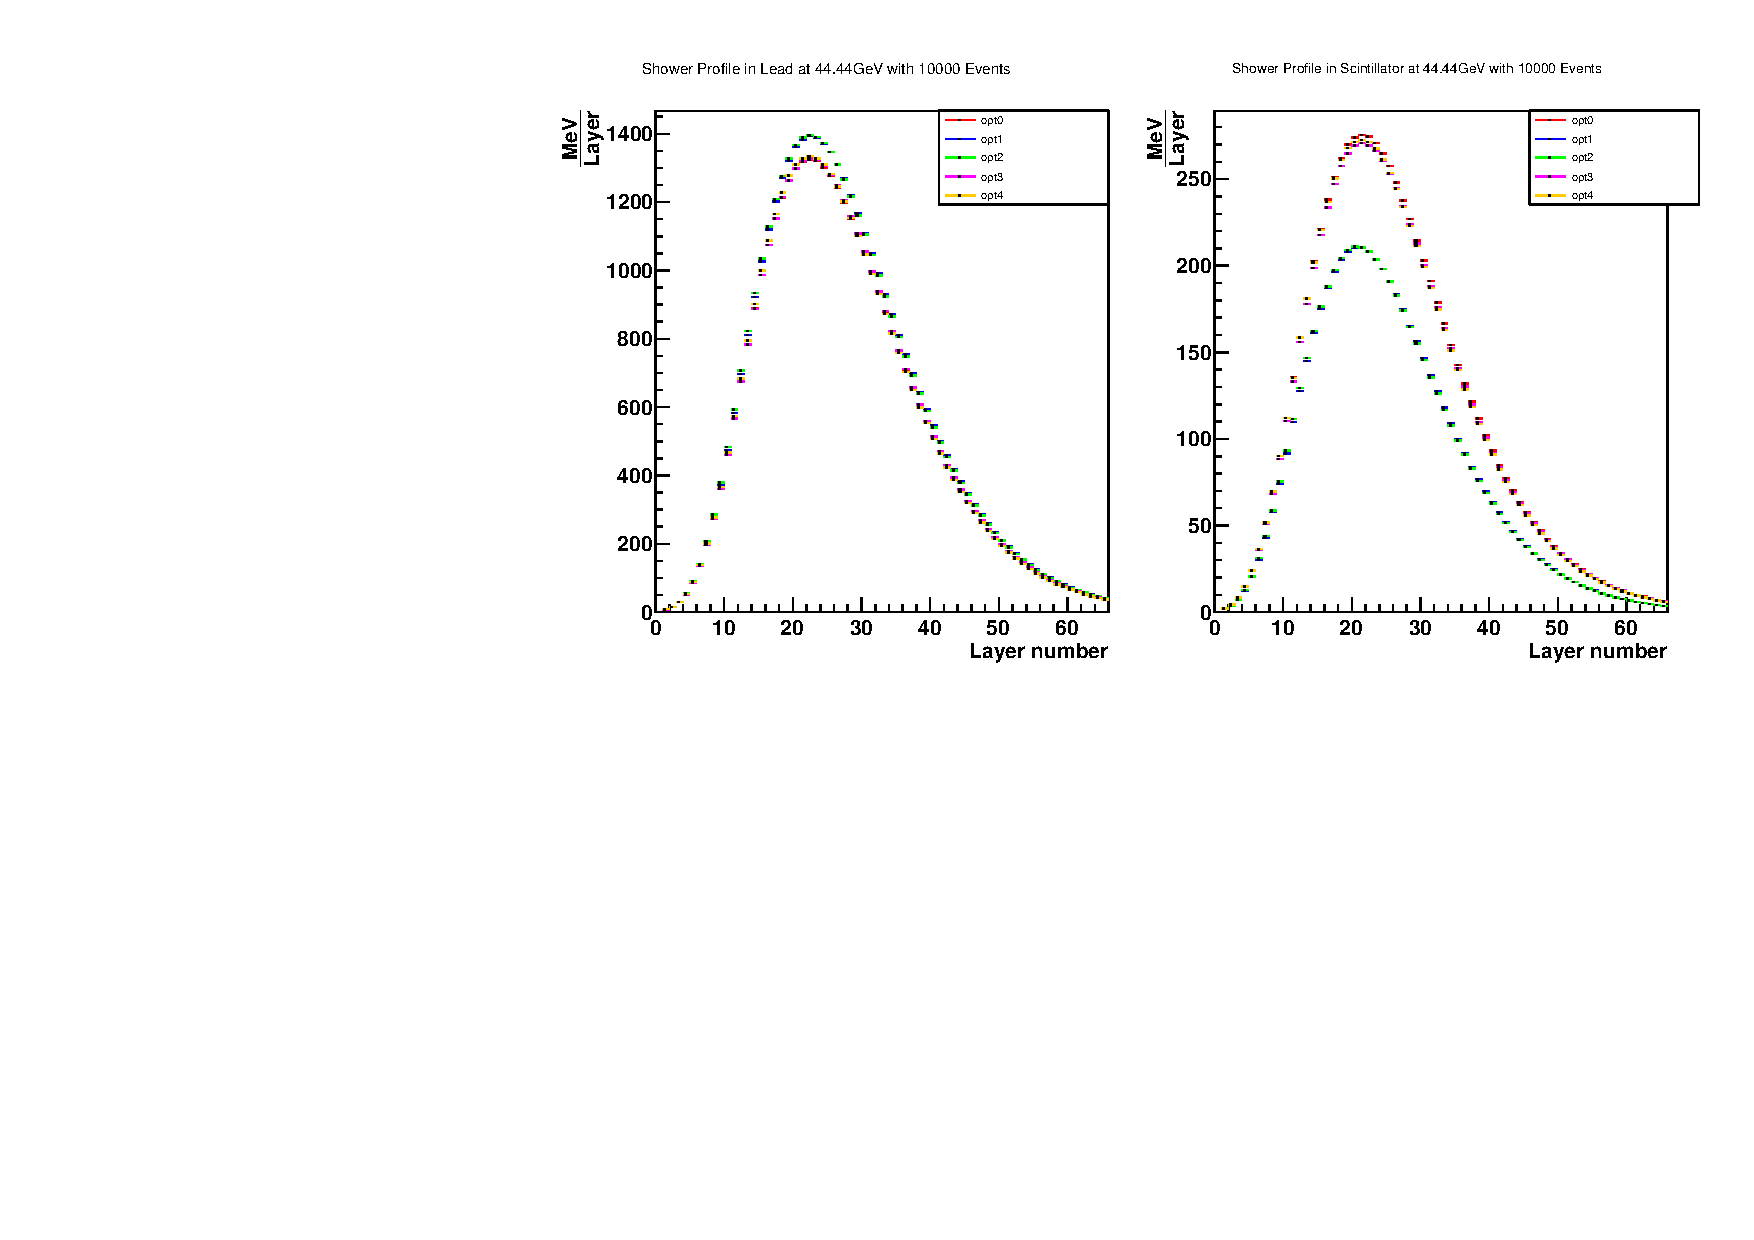
\includegraphics[width=\textwidth]{BoxShowers.pdf}
  \caption{Shower profiles in Lead and Scintillator layers of the ECAL using \geant supplied PLs}
  \label{fig:BoxPLShowers}
\end{figure}

Figure \ref{fig:BoxPLShowers} shows a comparison of shower profiles, in both mediums, for all of the \textit{emstandard} PLs.  This shows a significant discrepancy between PLs with and without a simplified multiple scattering model.  This is again useful confirmation that a simplified multiple scattering model does unfortuantely introduce bias to the results.


As in section \ref{sec:Sampling Fraction and Shower Profile Investigations} the shower profiles were integrated to obtain the sampling fraction and sampling ratio for each PL.
\begin{figure}[h]
  \centering
  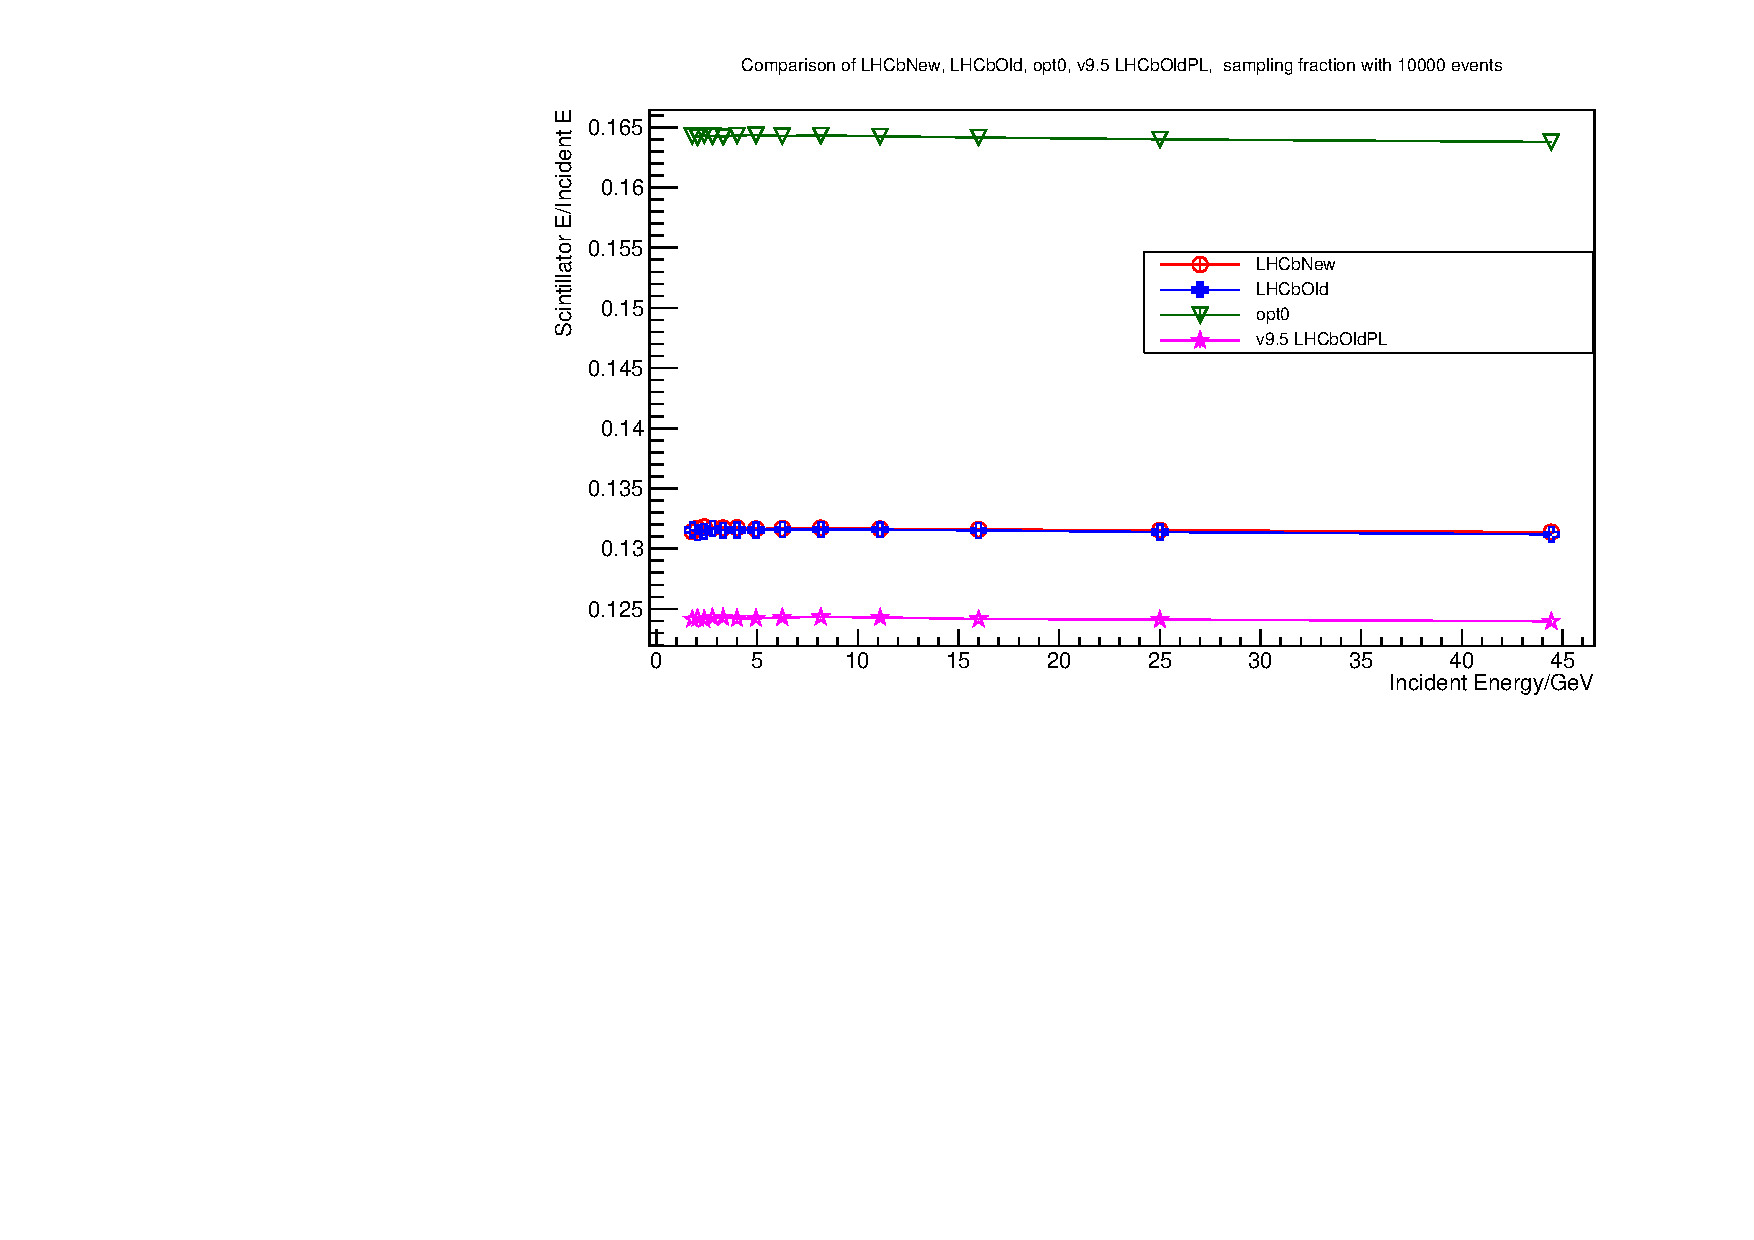
\includegraphics[width=\textwidth]{ProgressSF.pdf}
  \caption{Sampling fraction of the ECAL as a function of energy}
  \label{fig:ProgressSF}
\end{figure}
%\begin{figure}[h]
 % \centering
 % 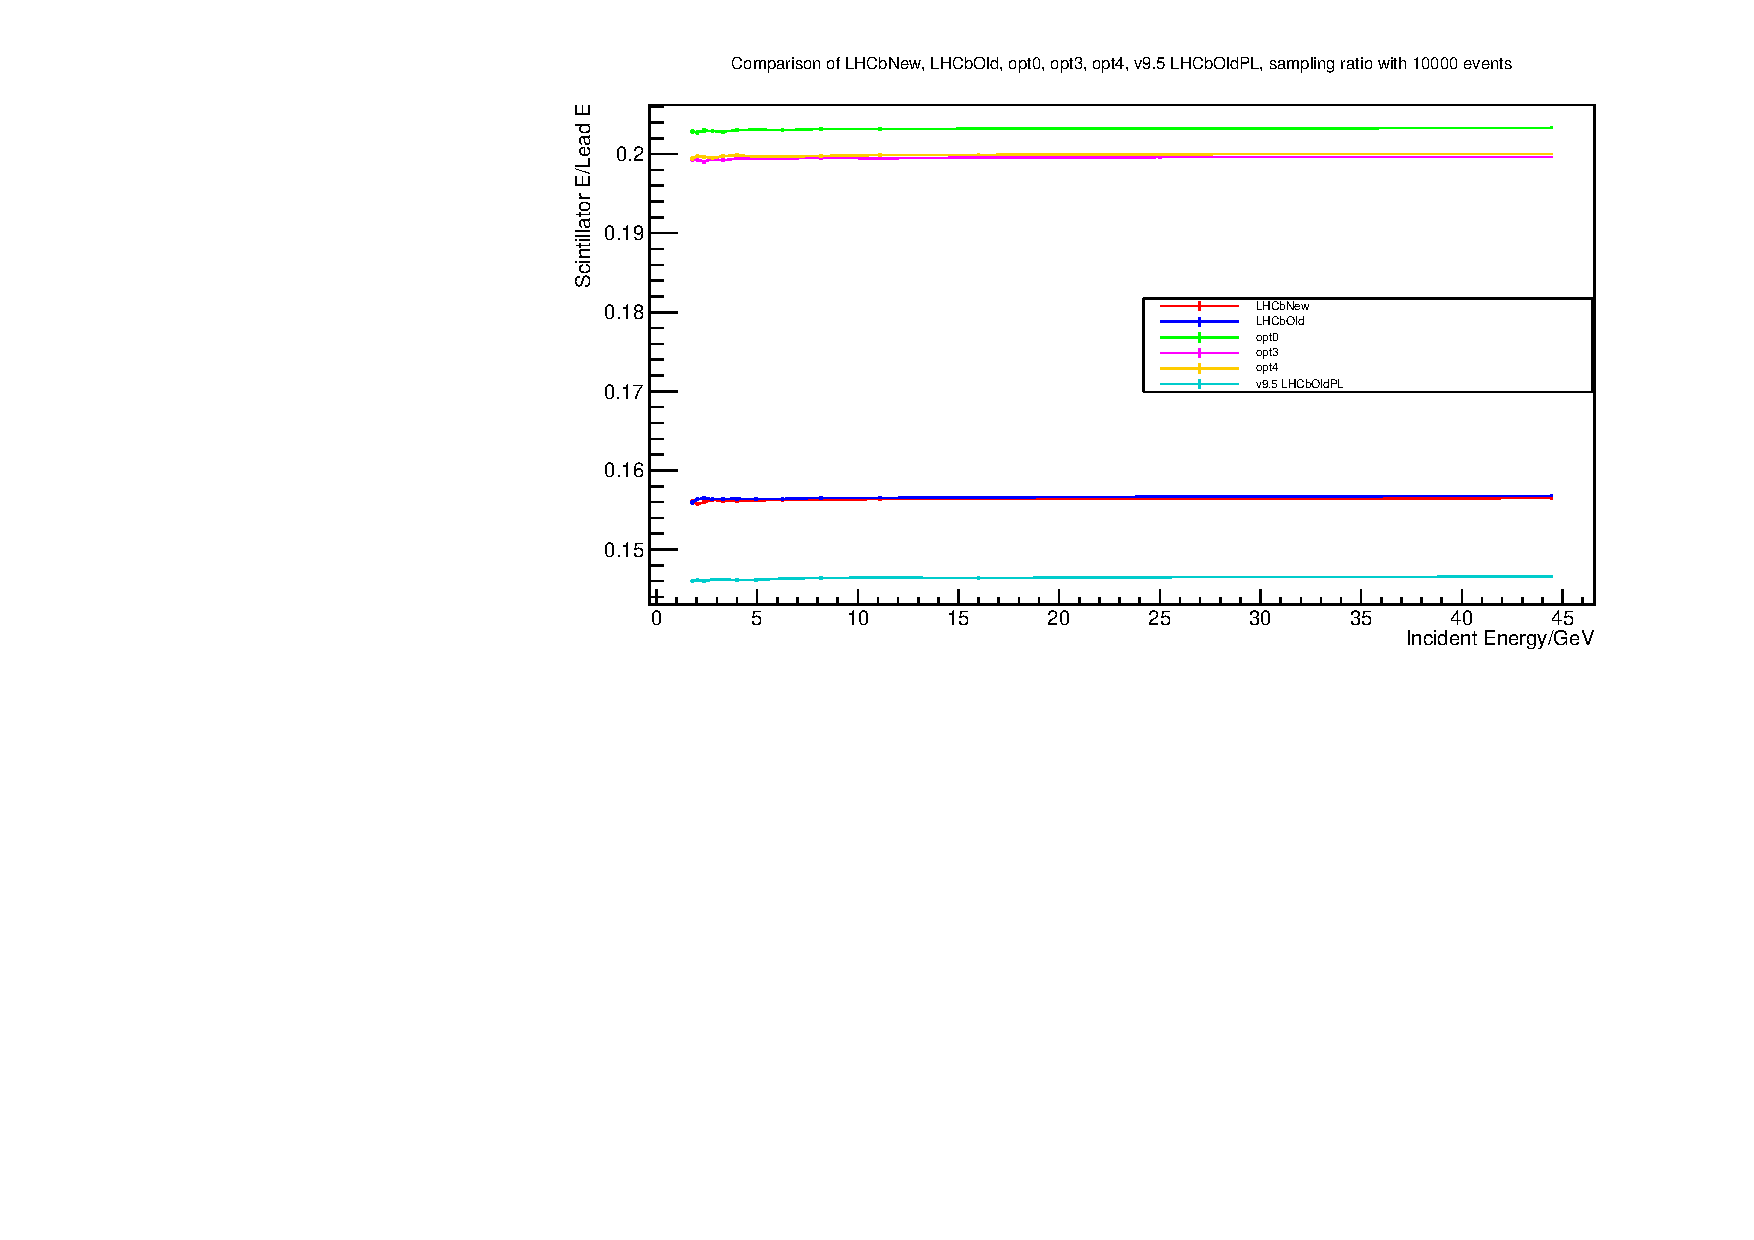
\includegraphics[width=\textwidth]{ProgressRatio.pdf}
 % \caption{Sampling ratio of the ECAL as a function of energy}
  %\label{fig:ProgressRatio}
%\end{figure}

Figure \ref{fig:ProgressSF} also shows that moving to \geant v9.6 has made progress towards more accurate results for the \lhcb private PLs.  Unlike the fractional resolution, however, the LHCbOld PL and LHCbNew PL sampling fractions are within uncertainties of each other at the majority of energies.  Therefore, for the purposes of choosing a new EM PL they have to be considered to be equally as accurate.

\begin{figure}[h]
  \centering
  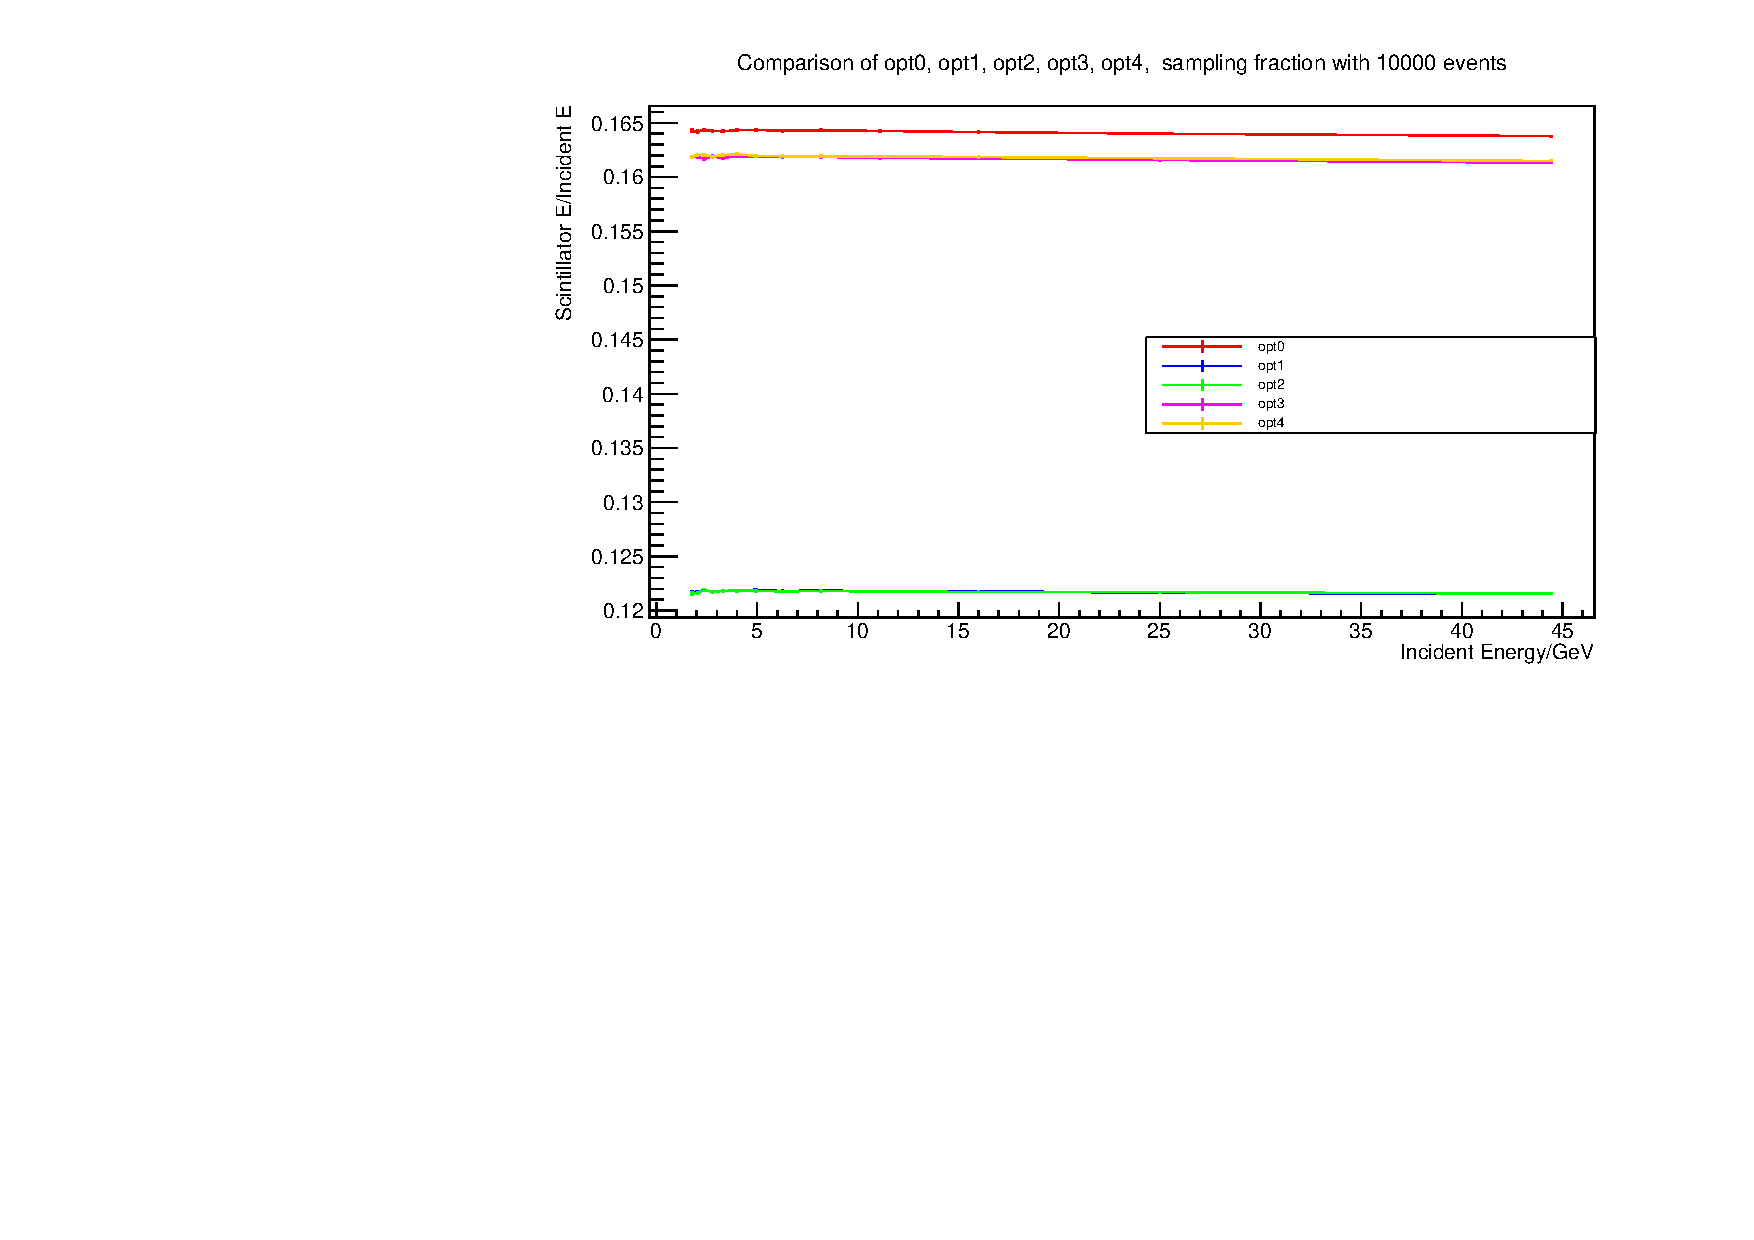
\includegraphics[width=\textwidth]{BoxSF.pdf}
  \caption{Comparison of sampling fractions from \geant supplied PLs}
  \label{fig:BoxSF}
\end{figure}
%\begin{figure}[h]
 % \centering
  %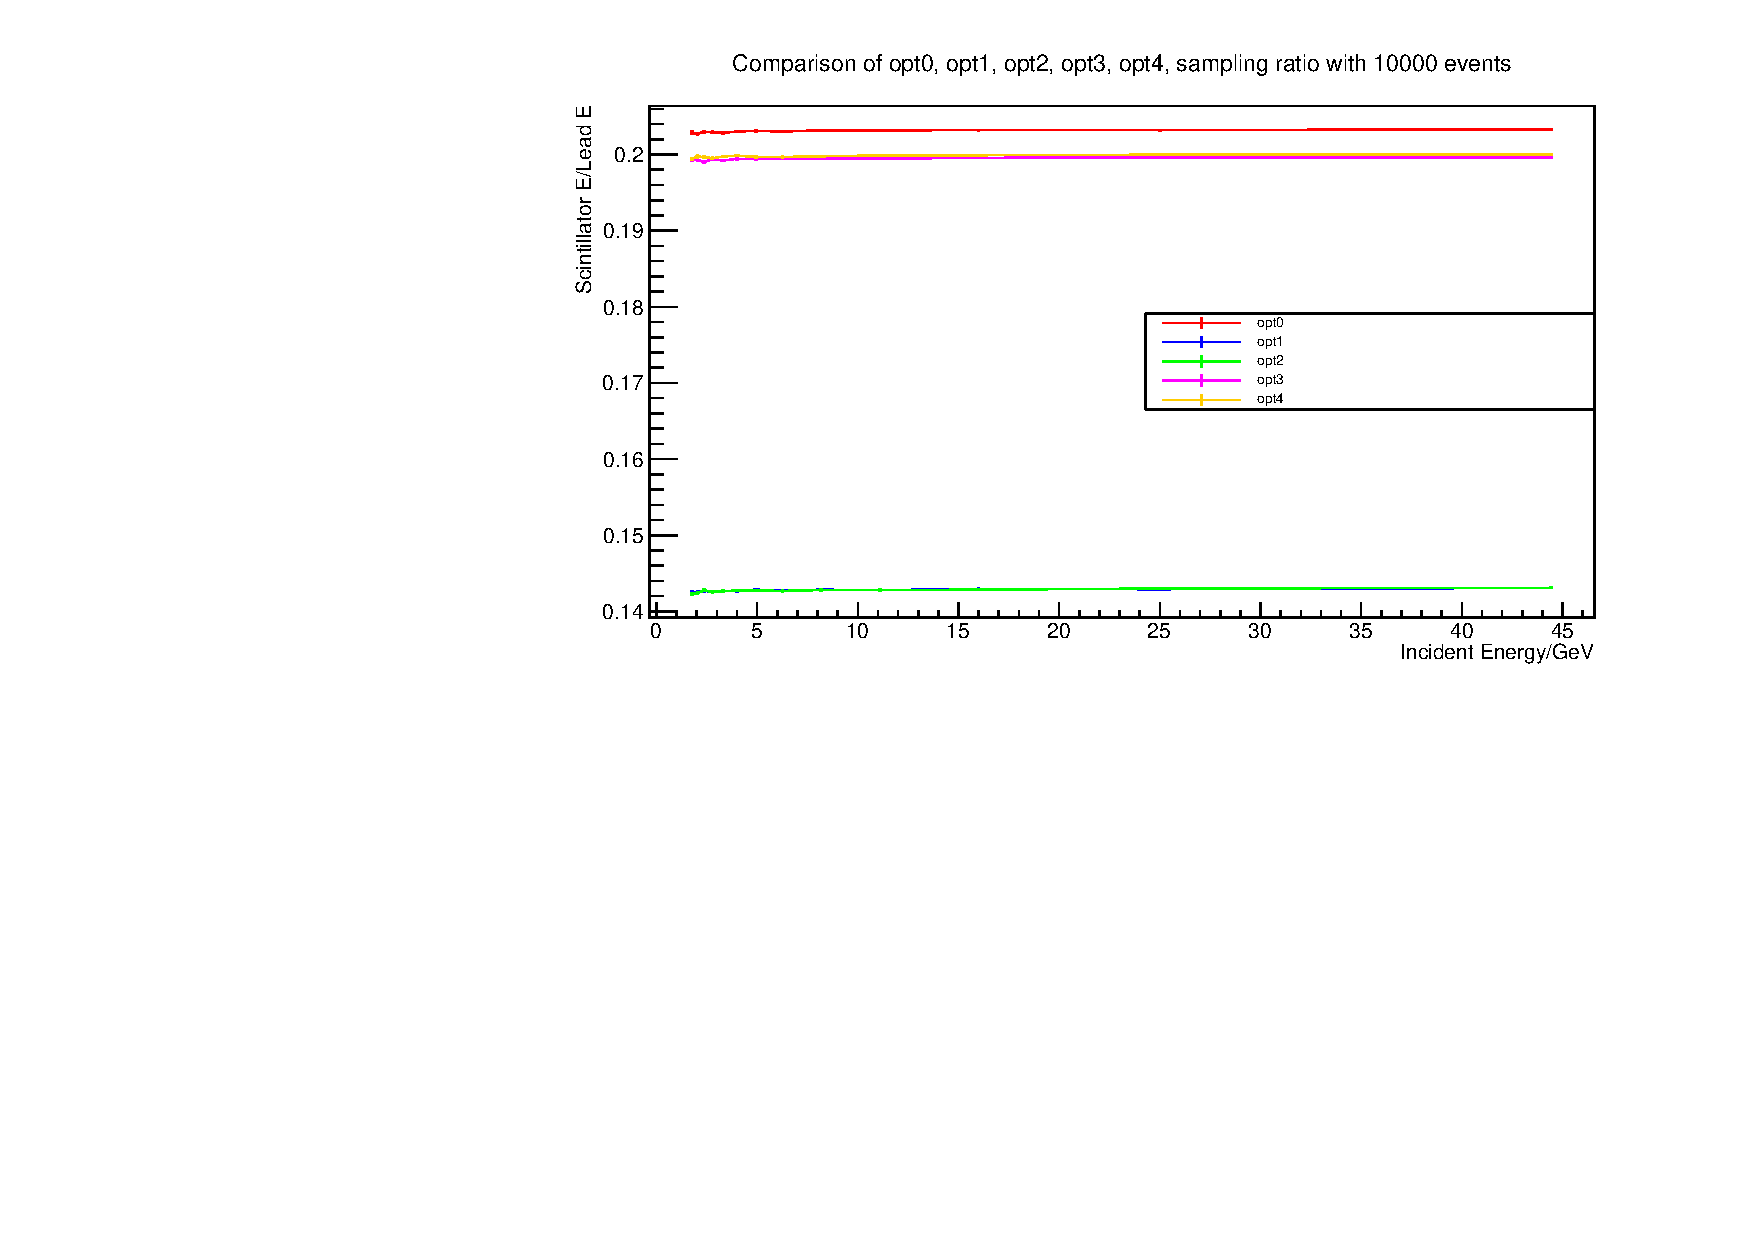
\includegraphics[width=\textwidth]{BoxRatio.pdf}
  %\caption{Comparison of sampling ratio from \geant supplied PLs}
  %\label{fig:BoxRatio}
%\end{figure}
Figure \ref{fig:BoxSF} shows that the \textit{opt1} and \textit{opt2} physics lists produce very similar results.  However, they are very different to the results produced by the more accurate PLs that do not use a simplified multiple scattering model.  The same effect is observed under \geant internal tests, which is a useful cross check\cite{1742-6596-219-3-032045}.

These results shows that using the \textit{fMimimal} option in the multiple scattering model has a large inpact on the amount of energy deposited, which is a quantity one would not intuitively expect to be effected by multiple scattering.  However, as described in section \ref{sec:steps}, the length of a step taken before all particle properties are re calculated is the minimium of the step length for all physics processes.  Consequently, the distance between positions where the energy loss is sampled can be effected by multiple scattering even though it plays no role in the energy loss calculations.  With \textit{fMinimal} applied the step lengths calculated for the multiple scattering process are longer, meaning that in some cases the step length used is also longer.  Therefore, energy losses are sampled less often which decreases the accuracy of the simulation.

\subsubsection{Simple Calorimeter Test Conclusions}
\label{ref:CaloConclusions}
Firstly, a significant discrepancy in fractional resolution and sampling fraction of a model \lhcb ECAL has been observed between \geant v9.5 and v9.6.  Consequently, the \lhcb calorimeter group will have to re calibrate the ECAL for the new release of \gauss. This discrepancy is believed to be a result of the new \geant version depositing more energy in scintillator and less in lead layers, most likely as a reuslt of updates to the multiple scattering models used.  This discrepancy has resulted in the \geant collaboration suggesting the \lhcb EM PL should be updated to a new multiple scattering model.  The studies in section \ref{sec:Comaprison of PL} show that updating the \lhcb EM PL to follow the \textit{emstandard opt1} PL actually increases this discrepancy. The stochastic component of the fractional resolution parameterisation changes from $0.922 \pm 0.0003$ with the old \lhcb PL to $0.910\pm 0.002$ with the updated \lhcb PL. However, the fractional resolution study using the most accurate PL available for the energy ranges considered here (\textit{emstandard opt0}) yields a stochastic term of $0.794\pm0.0002$.  Therefore, updating the \lhcb PL would cause progression of results towards a more accurate measurement.

A choice of PL has to be made for the next release of \gauss.  Throughout this study CPU time was monitored because it is a valuable and limited resource in particle physics.  It was noted that there was a siginificant increase in CPU time required when a PL without a simplified multiple scattering model was used. This increase varied from a factor of 2, to a factor of 6 compared to v9.5.  Other studies have shown that approximately $45\%$ of the time taken to simulate an event in \gauss is spent simulating the electromagnetic shower.  Therefore, even a factor of 2 increase in CPU time is not feasible.  The consequences of this are that only \textit{emstandard opt1}, \textit{emstandard opt2}, \textit{LHCbOld} and \textit{LHCbNew} are viable choices for the new PL.

Section \ref{sec:Comaprison of PL} shows that \textit{LHCbNew} produces results closest to un simplified multiple scattering models for fractional resolution studies.  Moreover, \textit{LHCbNew} and \textit{LHCbOld} both show closer agreement to the unbias PLs for sampling fractions and sampling resolutions compared to \textit{opt1} and \textit{opt2}.  Therefore, either of the \lhcb private PLs were deemed to be a better choice. 

Furthermore, \lhcb has previously experienced issues with the agreement between data and MC for the impact parameter resolution.  The conclusion of an extensive investigation into this issue was to use the PL described here as \textit{LHCbOld}.  Therefore, it was decided that the new PL should stay as close as possible to \textit{LHCbOld} to avoid introducing disagreements between data and MC elsewhere in the detector simulation.  Therefore, it was decided that the updated \lhcb private PL \textit{LHCbNew} should be adopted as the new EM PL.

%TODO cite geant4 testing.

%TODO cite jimmys thesis . 


%Figure \ref{fig:BoxPLStraightFR} shows 
%Simple Calorimeter Test
%----Calorimetry Background
%----Comparison of Geant4 versions
%---------Resolution investigations
%---------Sampling fraction investigations
%---------Geant4 version comparison results discussion
%----Physics List investigations
%---------Fractional Resolution
%---------Sampling Fraction Results
%---------Results Discussion

%MSC
%--results
\clearpage

\subsection{Multiple Scattering Test}
\label{sec:Multiple Scattering Test}
Since the multiple scattering model has been updated in the EM PL, it was decided a direct study of multiple scattering was necessary.  When a charged particle traverses a material there is a non-zero probability that it will undergo elastic coulomb scattering from a nuclei within the material.  The differential cross section for this process is given by,
\begin{equation}
  \label{eq:Rutherford}
  \frac{d\sigma}{d\Omega}=\big(\frac{1}{4\pi\epsilon_0}\big)^2\frac{z^2e^4}{M^2c^4\beta^4}\frac{1}{sin^4(\theta/2)}
  \end{equation}
where $\Omega$ is solid angle, z is the atomic number of the material, M is the mass of the charged particle and $\theta$ is the angle through which the charged particle is scattered\cite{eisberg1974quantum}.

Except for cases where the scattering material is a very thin film, the charged particle will scatter multiple times before exiting the material.  Hence, multiple coulomb scattering occurs which is more commonly known as just multiple scattering. The net effect is a lateral displacement as well as a scattering angle, as depicted in Figure \ref{fig:MSCPDG}.  In this case a statistical treatment has to be used to obtain a distibrution for the scattering angle, which is defined as $\theta$ in Figure \ref{fig:MSCPDG}. This was first carried out successfully by Moliere theory, which has been shown to give very good agreement with data over a wide range of particles, materials and energies \cite{PhysRev.89.1256,Gottschalk1993467}.  Several other theories have been shown to produce consistent results but the most complete is Lewis theory, which also provides moments for the spatial displacement distribution \cite{PhysRev.78.526}.

Both the Moliere and Lewis theory give a scattering angle distribution that is gaussian for the central $98\%$ of scattering angle values, but the tails of the distibrution fall off slower than a gaussian due to the $\frac{1}{sin^4(\theta/2)}$ term in equation \ref{eq:Rutherford}.  The width of the central gaussian is defined as $\theta_0$ which can be approximated by the Highland formula,
\begin{equation}
  \label{eq:Highland}
  \theta_0=\frac{14.1MeV}{pv}z\sqrt{\frac{L}{L_R}}\big[1+\frac{1}{9}log_{10}\big(\frac{L}{L_R}\big)\big]
\end{equation}
where p is the incident particles momentum, v is the incdient particles velocity, L is the length of the material and $L_r$ is the radiation length of the material.  This formula is an emperical formula that arises from fits to moliere theory \cite{Highland1975497}.

\begin{figure}[h]
  \centering
  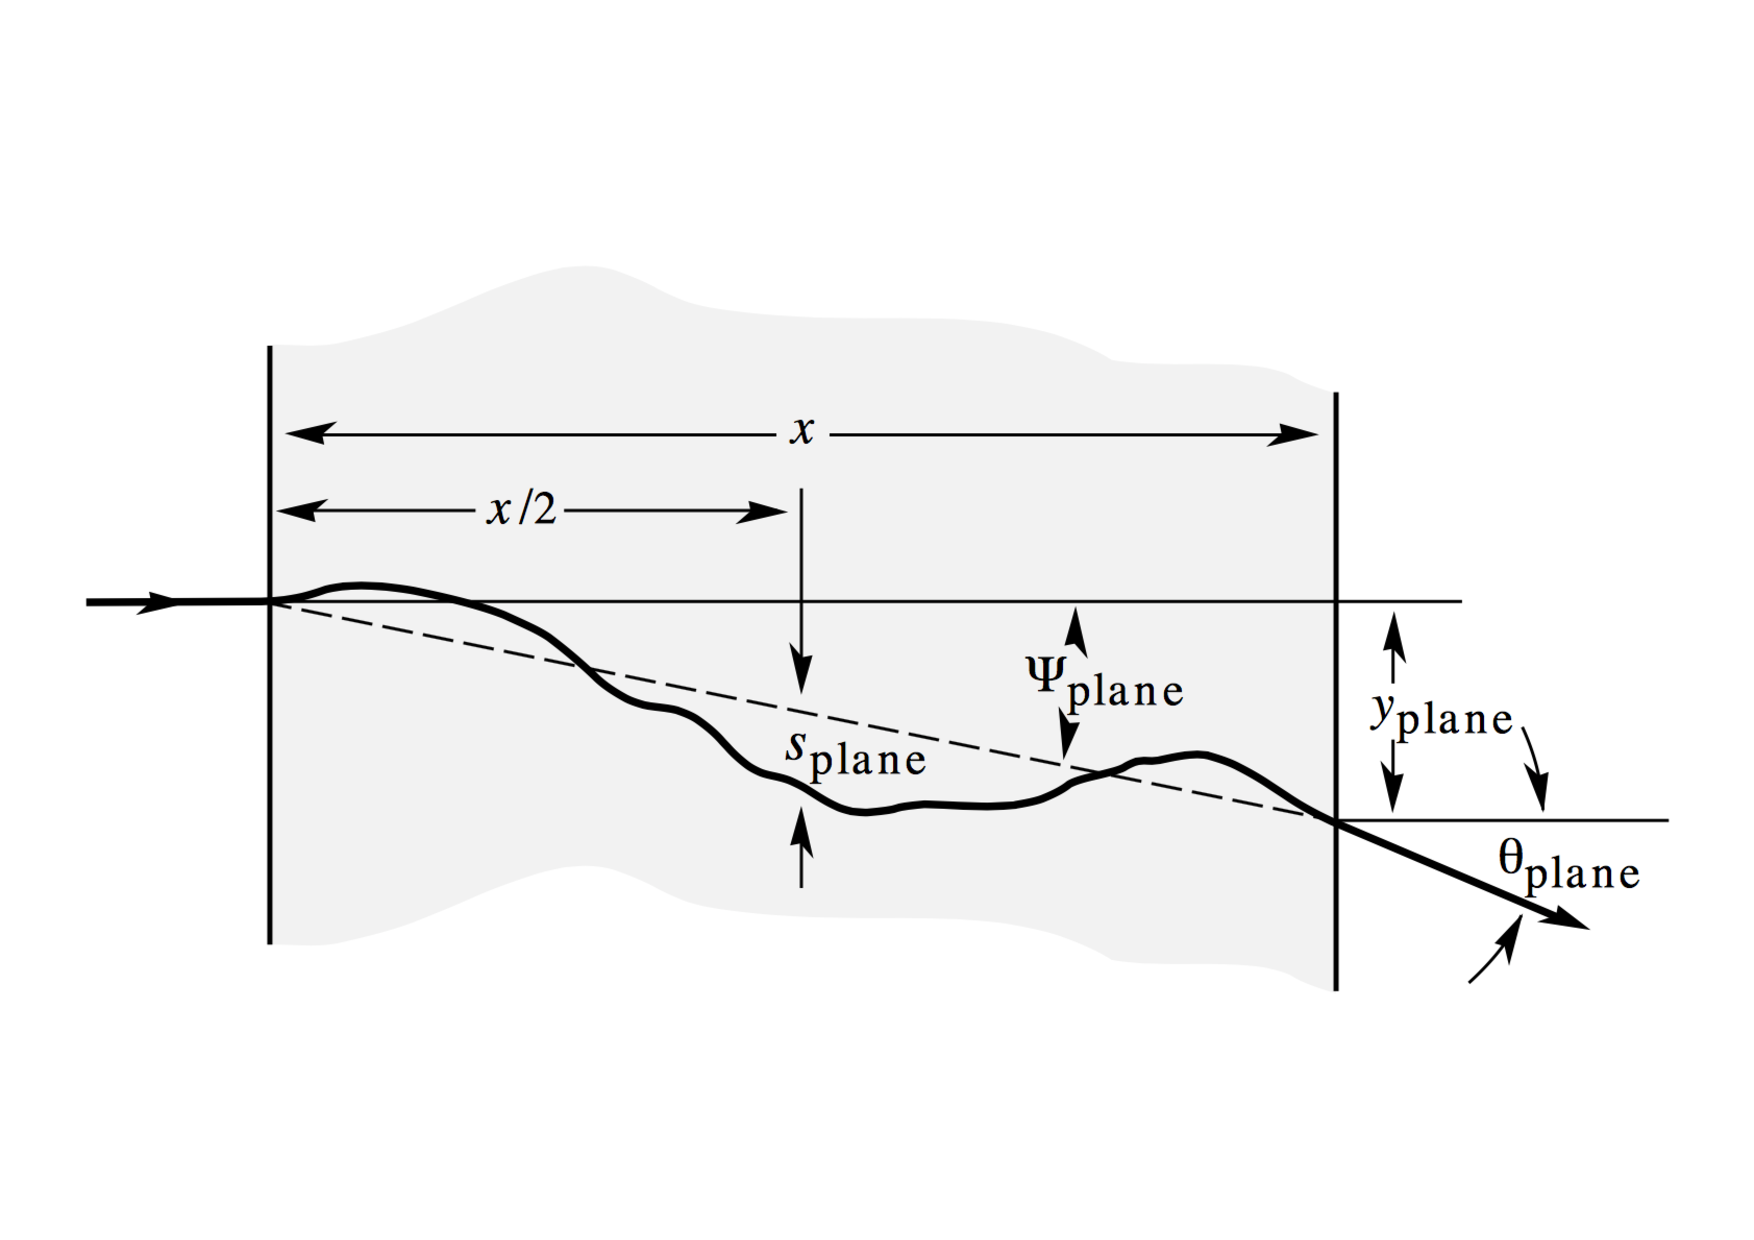
\includegraphics[width=\textwidth]{MSCPDG.pdf}
  \caption{A diagram showing the lateral displacement and angular dispersion when a charged particles traverses a medium.}
  \label{fig:MSCPDG}
\end{figure}

When one simulates multiple scattering, in a similar way to the theoretical models, it is rarely possible to simulate every individual collision.  It is only possible if the number of scatters is small and large amount of CPU time is available.  For the latter reason, this type of simulation based on simulating every single scatter was not implemented until 2005.  Unfortuantely, there is still a limited number of applications where this is a viable option.  The \textit{UrbanMsc} models get around this by using  a ``condensed'' simulation of multiple scattering, which involves simulating a step of the particles path at a time and applying net effects at the end of each step \cite{Urbàn:592633}.  More sepcifically, the angle through which the particle has been scattered and the lateral displacement are applied at the end of each step as part of the multiple scattering simulation.  The scattering angle is sampled from distributions calculated using Lewis theory but no theory of a full displacement distribution exists.  Therefore, \geant uses its own, non-exact, algorithms to calculate the lateral displacement after each step %TODO cite physics reference manual.

Another approach to simulating multiple scattering, that has been implemented more recently, is to use a ``mixed'' approach.  This involves sampling scatterers, where the scattering angle $\theta$ is below a threshold $\theta_{max}$, in a similar way to the ``condensed'' approach discussed previously.  However, if the scattering angle is above $\theta_{max}$ then a single scattering approach is used.  This is implemented in \geant as the \textit{WentzelVI} model.

In moving to the new EM PL the multiple scattering model for electrons and positrons has changed from \textit{UrbanMsc95} to \textit{WentzelVI} above 100MeV, therefore the model has moved from being condensed to mixed.  However, below 100MeV the model has moved from \textit{UrbanMsc95} to the older \textit{UrbanMsc93} which involves some subtle changes. %TODO write more.

To carry out a direct investigation of multiple scattering and how it is effected by these changes, the \geant example TestEm5 was used. The example provides the facility to fire particles into a square sheet of material at normal incidence and study the angle of the scattered particle, to the normal, as it exits the material on the other side. A diagram of this is shown in Figure \ref{fig:TestDiam}.  The type of material used, the width of the material and thickness of the material can all be specified. In this case the setup used was a $300 \mu m$ thick sheet of silicon designed to model the \lhcb VELO as closely as possible, because this is the area of the detector where the most precise tracking measurements sensitive to multiple scattering take place.
\begin{figure}[h]
  \centering
  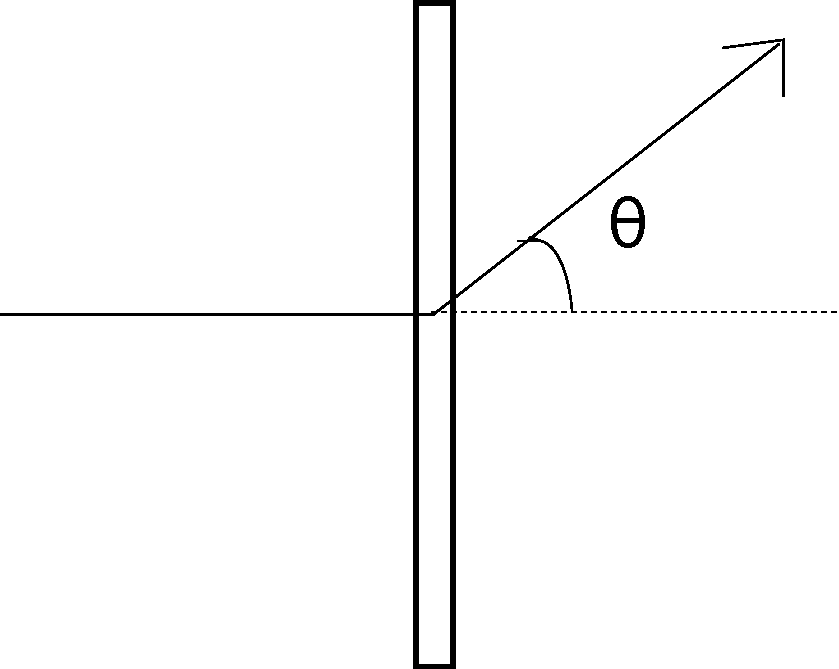
\includegraphics[width=0.7\textwidth]{TestEm5Diag.pdf}
  \caption{A diagram showing the setup of TestEm5.  $\theta$ is the angle under investigation by this test}
  \label{fig:TestDiam}
\end{figure}

The aim of this investigation was to measure the parameter $\theta_0$ of the scattered particles angular distribtuion for electrons at a range of energies and use it as a comparison tool between PL configurations and \geant versions.  The \geant example is pre-configured to calculate $\theta_0$ by taking the standard deviation of the central $98\%$ of values after each run.  However, no estimation of the uncertainty is performed by the example. As the time to simulate 10000 electrons with this minimal geometry was <1 second, the simulation was re-run 10000 times at each energy and configuration.  $\theta_0$ was recorded for each run and the end result was assigned as the mean of all runs with an uncertainty given by the RMS of all 10000 runs.

The energies chosen for this investigation were 1,2,3,4,5,7,9,12,15,20,25,30 and 40 GeV as these were considered representative of the expected electron energies at \lhcb. The following configurations were tested with these energies: \geant version 9.5 with the \textit{LHCbOld} PL and version 9.6 with \textit{LHCbNew} PL and verision 9.6 \textit{LHCbOld} PL.  These were chosen because it allows a direct comparison between the old release of \geant and the new release of \geant to be made.  v9.6 \textit{LHCbOld} was included to offer insight into the cause of any discrepancies observed.

\subsubsection{Results}
\label{sec:MscResults}
The results for $\theta_0$ from running the simulation with v9.6 \textit{LHCbOld} and \textit{LHCbNew} were divided by the results from running the simulation with v9.5 and \textit{LHCbOld} to make a direct comparison with the previous release of \geant.  These are shown in Figure \ref{fig:theta0}.


\clearpage
